\documentclass[11pt, headsepline, a4paper, fleqn, oneside]{article}
\usepackage{blindtext} 
\usepackage[french]{babel}
\usepackage[utf8x]{inputenc}
\usepackage{amsmath}
\usepackage{graphicx}
\usepackage[colorinlistoftodos]{todonotes}
\usepackage[margin=1.18in,article]{geometry}
%\usepackage{cmbright}
\usepackage{enumitem}
\usepackage{sidecap}
\usepackage{algorithm}
\usepackage[noend]{algpseudocode}
\usepackage{lmodern}
\usepackage{amssymb}
\usepackage{mathrsfs}
\usepackage[T1]{fontenc}
\usepackage{pifont}
\usepackage{color}
\usepackage{stmaryrd}
\usepackage{verbatim}
%\usepackage{fancyhdr}
\usepackage{tabularx}
\usepackage{listings}
\usepackage{tikz-cd}
\usepackage{hyperref}
\usepackage[noend]{algpseudocode}
\usepackage{subcaption}
\usepackage[normalem]{ulem}
\usepackage[nottoc,notlof,notlot]{tocbibind}
\usepackage[titles,subfigure]{tocloft}
\newtheorem{lem}{Lemme}
\newtheorem{prop}{Proposition}
\newtheorem{theo}{Théorème}
\newtheorem{defi}{Définition}
\newtheorem{coro}{Corollaire}
\newtheorem{propr}{Propriétés}
\newtheorem{rem}{Remarque}
\newtheorem{ex}{Exemple}
\newtheorem{rap}{Rappel}
\newtheorem{Bilan}{Bilan}
\newtheorem{app}{\color{gris}Application}
\newtheorem{nota}{\color{cyan}Notation}
\newtheorem{demo}{Preuve}
\usepackage{cleveref}
\definecolor{trolleygrey}{rgb}{0.5, 0.5, 0.5}
\newcommand{\Z}{\mathbb{Z}}
\newcommand{\F}{\mathbb{F}_q}
\newcommand{\N}{\mathbb{N}}
\newcommand{\R}{\mathbb{R}}
\newcommand{\K}{\mathbb{K}}
\newcommand{\E}{\mathcal{E}}
\newcommand{\q}{\bar{q}}
\definecolor{turquoise}{rgb}{0.19, 0.84, 0.78}
\definecolor{cobalt}{rgb}{0.0, 0.28, 0.67}
\definecolor{calpolypomonagreen}{rgb}{0.12, 0.3, 0.17}
\usetikzlibrary{arrows}
\tikzset{
  treenode/.style = {align=center, inner sep=0pt, text centered,
    font=\sffamily},
  arn_n/.style = {treenode, circle, white, font=\sffamily\bfseries, draw=black,
    fill=black, text width=1.5em},% arbre rouge noir, noeud noir
  arn_r/.style = {treenode, circle, red, draw=red, 
    text width=1.5em, very thick},% arbre rouge noir, noeud rouge
  arn_x/.style = {treenode, rectangle, draw=black,
    minimum width=0.5em, minimum height=0.5em}% arbre rouge noir, nil
}
\begin{document}

%\pagestyle{fancy}
\begin{titlepage}

\newcommand{\HRule}{\rule{\linewidth}{1mm}} % Defines a new command for the horizontal lines, change thickness here

\center 
 
%----------------------------------------------------------------------------------------
%	HEADING SECTIONS
%----------------------------------------------------------------------------------------

% Name of your university/college
\begin{minipage}{1\textwidth}
\centering
\textsc{\LARGE Université Paris-Saclay UVSQ}\\[0.5cm] 

\includegraphics[scale=0.13]{versailles.jpg} 
\end{minipage}
\\[1.5cm]
\textsc{\Large Rapport de stage }\\[0.5cm] % Major heading such as course name
\textsc{\large Master d'algèbre appliquée à la cryptographie}\\[0.5cm] % Minor heading such as course title

%----------------------------------------------------------------------------------------
%	TITLE SECTION
%----------------------------------------------------------------------------------------

\HRule \\[0.4cm]
{ \huge Développement de méthodes d'optimisation de circuits booléens pour la cryptographie homomorphe}\\[0.1cm] % Title of your document
\HRule \\[1cm]
 
%----------------------------------------------------------------------------------------
%	AUTHOR SECTION
%----------------------------------------------------------------------------------------

\begin{minipage}{0.3\textwidth}
\begin{center} 
\textbf{Auteur:}\\
Abdessamad \textsc{Fazzat} 

\end{center}
\end{minipage}
~
\begin{minipage}{0.3\textwidth}
\begin{center} 
\textbf{Tuteurs:} \\
Pascal \textsc{Aubry}\,,
Sergiu \textsc{Carpov}
\end{center}
\end{minipage}
~
\begin{minipage}{0.3\textwidth}
\begin{center} 
\textbf{Encadrant:} \\
Louis \textsc{Goubin} 
\end{center}
\end{minipage}\\[2cm]
%----------------------------------------------------------------------------------------
%	DATE SECTION
%----------------------------------------------------------------------------------------
\center {\large \today}\\[2cm]
%----------------------------------------------------------------------------------------
%	LOGO SECTION
%----------------------------------------------------------------------------------------


\begin{minipage}{0.5\textwidth}
\centering

\includegraphics[scale=0.14]{logo-cea.png} 
\end{minipage}


%----------------------------------------------------------------------------------------


\vfill %

\end{titlepage}

\tableofcontents
\newpage
\section{Présentation de l'entreprise}

\paragraph{Présentation du CEA}: \\
Créé il y a plus de 70 ans, le CEA\footnote{Commissariat à l'énergie atomique et aux énergies alternatives: \url{http://www.cea.fr/}} est un organisme public de recherche à caractère scientifique, technique et industriel (EPIC).\\
Acteur majeur de la recherche, du développement et de l'innovation, le CEA intervient dans quatre domaines: la défense et la sécurité, les énergies bas carbone (nucléaire et renouvelables), la recherche technologique pour l'industrie et la recherche fondamentale (sciences de la matière et sciences de la vie). S'appuyant sur une capacité d'expertise reconnue, le CEA participe à la mise en place de projets de collaboration avec de nombreux partenaires académiques et industriels.
\begin{figure}[ht]
    \centering
    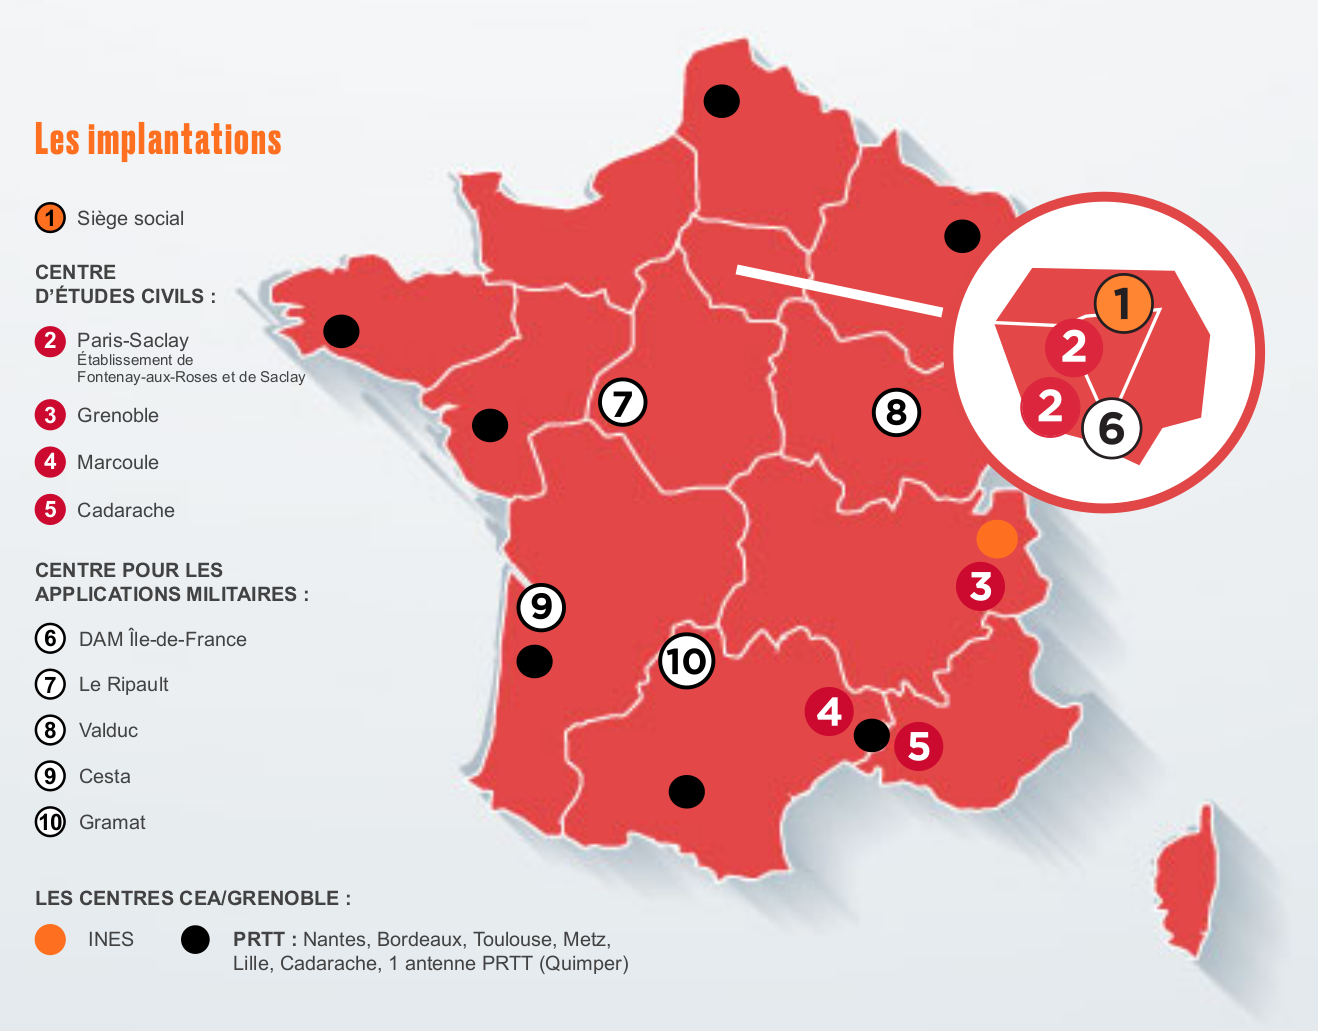
\includegraphics[width = 0.6\linewidth]{cea.png}
    \caption{Implantations géographiques du CEA}
\end{figure}
\paragraph{La direction de la recherche technologique (DRT, Cea-Tech)}:\\
La DRT\footnote{\url{http://www.cea-tech.fr/cea-tech}} a pour mission de contribuer à la compétitivité des entreprises françaises via le développement technologique et le transfert de connaissances, de compétences et de technologies, elle compte 4000 personnes basées à Grenoble, Saclay et au sein des plateformes régionales de transfert technologique (PRTT). CEA Tech est constituée des trois instituts Leti, Liten, List et de l’institut CEA Tech en région, qui lui permettent de disposer d’un portefeuille de technologies complet dans les domaines de l’information et de la communication, de l’énergie et de la santé.
\paragraph{Institut List}:\\
Ce stage à été effectué au sein de l'équipe CRYPTO du Laboratoire Composants Logiciels pour Sûreté et Sécurité des Systèmes (L3S) de l'institut List\footnote{Laboratoire d'Intégration de Systèmes et des Technologies: \url{http://www-list.cea.fr/}}, dans le Département Architecture, Conception et Logiciels Embarqués (DACLE).

\section{Introduction et objectifs}

\paragraph{Introduction générale}:\\ 

La cryptographie utilisée actuellement repose principalement sur deux problèmes mathématiques : la factorisation et le logarithme discret. Mais on s'intéresse maintenant à d'autres alternatives qui pourraient, par exemple prétendre résister à l’ordinateur quantique. L'une de ces alternatives, offrant de nouvelles perspectives dont le chiffrement homomorphe, repose sur la géométrie des réseaux euclidiens, cette méthode s'est imposée durant cette dernière décennie de recherche.\\

Le chiffrement homomorphe est apparu pour la première fois en 2009 avec les travaux de Carlos Aguilar et de Craig Gentry \cite{homenc}. L'objectif étant de pouvoir manipuler des données sans avoir à les déchiffrer. Cependant, le caractère homomorphe de certains schémas de chiffrement n'est pas récent, le schéma RSA datant de 1977 est homomorphe pour la multiplication et le schéma de Pailler datant de 1999 l'est pour l'addition. En revanche, la vraie révolution des travaux datant de 2009 est le chiffrement complètement homomorphe, permettant de faire des calculs arbitraires sur des données chiffrées. Bien que cette nouvelle construction requiert de tels paramètres qu'elle est inutilisable en pratique.
ce type de chiffrement pourrait devenir indispensable, surtout avec l'apparition du Cloud-Computing, et offre des solutions pour des problèmes récents de la cryptographie, comme le vote électronique ou encore le calcul multipartite sécurisé.

Une nouvelle révolution pour ce type de chiffrement est l'arrivée des schémas tels que Brakerski-Gentry-Vaikuntanathan (BGV), Fan-Vercauteren (FV) ou Brakerski \og scale invariant \fg, dont la sécurité est directement liée au problème Learning With Errors (LWE).\\

\paragraph{Objectifs du stage}:\\

Pour aider le développeur à utiliser cette technologie, le CEA LIST a développé l’outil Open source \textsc{Cingulata} qui permet d’exécuter homomorphiquement des programmes écrits dans un langage de haut niveau (C++). En effet, cet outil permet de transformer le code source de haut niveau dans un circuit booléen équivalent et d’exécuter ce circuit sur des données chiffrées. Grâce à cet outil, certaines entreprises peuvent ainsi fournir des services sur des données d’utilisateurs tout en préservant leur vie privée. Ces méthodes intéressent différents domaines d’application, tels que médical, l'industrie du futur ou la publicité ciblée. Néanmoins, les performances des implémentations actuelles ne permettent pas encore de pouvoir déployer ces services à grande échelle. En effet, les calculs en homomorphe induisent par construction du bruit. Ce bruit tend à augmenter avec la complexité des calculs effectués jusqu'à atteindre une certaine taille au delà de laquelle il ne sera plus possible de déchiffrer le message correctement.\\
....
\section{Préliminaires}
\subsection{Rappels et notations}
Pour décrire la répartition des valeurs que peut prendre une variable aléatoire, on lui associe une loi de probabilité (ou distribution), elle se caractérise par sa fonction de distribution cumulative (CDF) $F_{X}(x)=P(X \leq x)=P\left(X_{1} \leq x_{1}, \cdots, X_{n} \leq x_{n}\right)$. Si la variable est discrète alors sa loi est déterminée par la probabilité de chacune des valeurs qu'elle peut prendre et par une fonction de densité de probabilité (PDF) si elle est continue, cette fonction est la dérivée de la CDF.

\begin{defi}[Loi normale] ou $\bold{Gaussienne}$, qu'on note souvent par $\mathcal{N}(c,\sigma^2)$, est caractérisée par son centre $c$ et écart type $\sigma$ et sa densité de probabilité est donnée par 
\begin{equation}
    f(x)=\frac{1}{\sigma \sqrt{2 \pi}} \exp(-\frac{(x-c)^{2}}{2 \sigma^{2}})
\end{equation}
\end{defi}
On dit qu'une variable aléatoire $X$ de $\R$ est une $\sigma$-sous-gaussienne si pour tout $r\in \R$ $
\mathbb{E}[\exp (r X)] \leq \exp \left(\frac{\sigma^{2} r^{2}}{2}\right)
$, où $\mathbb{E}[X]$ est l'espérance de $X$.\\
De manière équivalente, comme la probabilité $\mathbb{P}[X>x]=\mathbb{P}\left[\exp (r X)>e^{r x}\right] \leq \frac{\mathbb{E}[\exp (r X)]}{e^{r x}}$ et $X$ est $\sigma$-sous-gaussienne, on obtient $\mathbb{P}[X>x] \leq \exp \left(\frac{x^{2} \sigma^{2}}{2}-r x\right)$. Le terme à l'intérieur de l'exponentielle (comme fonction en $x$) est minimal pour $x=r / \sigma^{2}$, d'où:
\begin{equation}
    \forall x>0,\,
\mathbb{P}[X>x] \leq \exp \left(-\frac{x^{2}}{2 \sigma^{2}}\right)
\end{equation}

\begin{lem}\label{lem1}
Soient $(X_i)_{1\leq i\leq n}$ des variables aléatoires indépendantes telles que $X_i$ soit $\sigma_i$-sous-gaussienne. Alors pour tout $\lambda_1,\dots,\lambda_n \in \R$, la variable aléatoire $X=\lambda_1 X_1 +\dots+\lambda_n X_n$ est $\sigma$-sous-gaussienne, avec $\sigma^{2}=\lambda_{1}^{2} \sigma_{1}^{2}+\cdots+\lambda_{n}^{2} \sigma_{n}^{2}$.
\end{lem}

%\begin{demo} Comme les $X_i$ sont indépendantes, on a pour tout $r\in \R$
%$$\begin{aligned} \mathbb{E}[\exp (r X)] &=\mathbb{E}\left[\exp %\left(r\left(\lambda_{1} X_{1}+\cdots+\lambda_{n} X_{n}\right)\right)\right] \\ %&=\mathbb{E}\left[\exp \left(\lambda_{1} r X_{1}\right) \cdots \exp %\left(\lambda_{n} r X_{n}\right)\right]=\prod_{i=1}^{n}\mathbb{E}\left[\exp %\left(\lambda_{i} r X_{i}\right)\right] \end{aligned}$$
%et comme elles sont $\sigma_i$-sous-gaussiennes, on a $\mathbb{E}\left[\exp %\left(\lambda_{i} r X_{i}\right)\right] \leq \exp \left(\frac{x^{2}\left(\lambda_{i} \sigma_{i}\right)^{2}}{2}\right)$ et on en %déduit pour tout $i$
%$$
%\mathbb{E}[\exp (r X)] \leq \prod_{i=1}^{n} \exp %\left(\frac{r^{2}\left(\lambda_{i} \sigma_{i}\right)^{2}}{2}\right)=\exp %\left(\frac{r^{2} \sigma^{2}}{2}\right)
%$$
%avec $\sigma^{2}=\lambda_{1}^{2} \sigma_{1}^{2}+\cdots+\lambda_{n}^{2} %\sigma_{n}^{2}$
%\end{demo}

Soient $X,\,Y$ deux variables aléatoires indépendantes de PDF $f_X$ et $f_Y$ respectivement, on pose $V=XY$ et on a le résultat suivant sur la loi de $V$

\begin{theo}
\begin{equation}
    f_V (v) = \int_{-\infty}^{+\infty} \frac{1}{|x|} f_X (v/x)f_Y (x) \mathrm{d}x 
\end{equation}
\end{theo}

\subsection{Learning With Errors}
L'apprentissage avec erreurs, souvent abrégé LWE (Learning With Errors) est un problème calculatoire introduit par Oded Regev \cite{Regev10} reposant sur les réseaux euclidiens et qui est conjecturé difficile, à partir duquel est construite une grande partie des schémas de chiffrement homomorphes.
Ce problème repose sur la difficulté de retrouver un vecteur secret $\boldsymbol{s} \in \Z_q ^n$, connaissant plusieurs entrées $\{(\boldsymbol{a},\langle\boldsymbol{a}, \boldsymbol{s}\rangle+ e)\}$ où $\langle , \rangle$ est le produit scalaire et $e$ un bruit tiré de distributions appropriées. Cependant, retrouver $\boldsymbol{s}$ si l'on possède des produits scalaires $\langle\boldsymbol{a}, \boldsymbol{s}\rangle$ et suffisamment de vecteurs $\boldsymbol{a}$, est un problème d'algèbre linéaire facile à résoudre (Pivot de Gauss, bases de Gröbner, $\dots$). \\
Formellement, pour un module $q$ polynômial en la taille de $n$, résoudre le problème LWE revient à trouver une solution pour un système d'équations approximatives (bruité):
$$
\begin{aligned}\left\langle\boldsymbol{s}, \boldsymbol{a}_{1}\right\rangle & \approx_{\chi_{err}} \ b_{1} \bmod q \\\left\langle\boldsymbol{s}, \boldsymbol{a}_{2}\right\rangle & \approx_{\chi_{err}} \ b_{2} \bmod q \\ \vdots \end{aligned}
$$
\begin{rem}
Le cas $q=2$ correspond au Learning Parity with Noise (LPN)
\end{rem}
Soit $\rho(x)=\exp \left(-\pi x^{2}\right)$ pour $x \in \mathbb{R} .$ On définit la fonction Gaussienne $$\rho_{c, \sigma}(x)=\rho(\|x-c\| / \sigma)$$ de paramètres $c,\,\sigma$, qu'on étend sur tout ensemble $M$ de $\R$ par $\rho_{c, \sigma}(M)=\sum_{k \in M} \rho_{c, \sigma}(k)$.
Considérons la distribution Gaussienne discrète suivante, définie pour tout entier $x$ par
$$
D_{\Z, \sigma, c}(x)=\frac{\rho_{c, \sigma}(x)}{\rho_{c, \sigma}(\Z)} =\frac{\exp \left(-\pi\|x-c\|^{2} / \sigma^{2}\right)}{\sum_{k \in \mathbb{Z}} \exp \left(-\pi\|x-c\|^{2} / \sigma^{2}\right)}
$$

\begin{defi}[Distribution LWE]
soient $n \geq 1, q \geq 2$ et un paramètre réel $\alpha \in[0,1]$, pour un vecteur secret $\boldsymbol{s}\in \Z_q ^n$, la distribution LWE $D_{n,q,\alpha}(\boldsymbol{s})$ définie sur $\Z_{q}^{n} \times \Z_{q}$ en choisissant uniformément $\boldsymbol{a} \leftarrow  \mathbb{Z}_{q}^{n}$ et $e \leftarrow D_{\mathbb{Z}, \alpha \cdot q, 0}$ $(=\chi_{err})$ puis en retournant le couple $(\boldsymbol{a}, b=\langle\boldsymbol{s}, \boldsymbol{a}\rangle+ e \bmod q)$.
\end{defi}
Cela nous permet de définir les deux problèmes suivants.
\begin{defi}[Le problème de recherche LWE]
étant donnés des échantillons selon une distribution LWE, retrouver $\boldsymbol{s}$.
\end{defi}
\begin{defi}[Le problème de décision LWE]
distinguer la distribution LWE $D_{n,q,\alpha}(\boldsymbol{s})$ pour $\boldsymbol{s}\in \Z_q ^n$ fixé, de la distribution uniforme de $\Z_{q}^{n} \times \Z_{q}$.
\end{defi}
Notons que le bruit $e$, comme défini par Regev, dépend du paramètre $\alpha$ de manière que $\chi_{err}$ soit d'écart type $\alpha q$. Prenons par exemple $\alpha = 0$, cela signifie l'absence du bruit et on peut donc retrouver le secret en temps polynômial.

\subsection{Ring Learning With Errors}
La nécessité d’utiliser des vecteurs de grande taille avec de gros coefficients, afin d'aboutir à des schémas avec des niveaux de sécurité suffisants, rend le LWE inefficace en pratique, c'est pourquoi Lyubashevsky, Peikert et Regev ont introduit une nouvelle variante sur les anneaux, le Ring Learning With Errors RLWE, reposant sur les réseaux idéaux.
Notons que le système d'équations approximatives (ou bruitées) dans le cas du LWE nous fournit une matrice $A$ de taille $n\times n$, cette matrice est remplacée dans la variante RLWE par un élément $\boldsymbol{a}$ de $\mathcal{R}_q$ à $n$ coefficients au lieu de $n^2$. En d'autres termes, cette structure d'anneau permet aux systèmes de chiffrement reposant sur le problème LWE de diminuer la taille de la clé publique. 
\begin{defi}
Pour un entier naturel $m\geq 1$, le polynôme \ $ \mathbf{\Phi}_{m}(X)=\prod_{1 \leq k<m \atop k \wedge m=1}\left(X-\zeta_{m}^{k}\right)$ est appelé le $m$-ième polynôme cyclotomique, de degré $\varphi(m)=n$ et qui vérifie:
$$X^{m}-1=\prod_{d | m} \mathbf{\Phi}_{d}(X)$$
Où $\zeta_{m}$ est une racine primitive $m$-ième de l'unité.
\end{defi}

Soit $\mathcal{R}=\mathbb{Z}[X] /\langle \mathbf{\Phi}_{m}(X)\rangle$ l'anneau des polynômes à coefficients entiers, modulo $\mathbf{\Phi}_{m}(X)$, avec $n$ une puissance de $2$. Les éléments de $\mathcal{R}$ seront représentés dans la base $\left\{1, X, \ldots X^{n-1}\right\}$ et pour $\boldsymbol{a}=\sum_{i=0}^{n-1} a_{i} X^{i} \in \mathbb{Z}[X]$, on note $\|\boldsymbol{a}\|_{\infty}=\max \left\{\left|a_{i}\right|, 0 \leqslant i<n\right\}$ sa norme infinie.
Soit $t$ le module de l'anneau des messages clairs $\mathcal{R}_t=\mathcal{R} /t \mathcal{R}$ et $q$ celui de l'anneau des messages chiffrés $\mathcal{R}_q\times \mathcal{R}_q$, avec $q\gg t$.
On note $\mathcal{U}$ la distribution uniforme de $\mathcal{R}_q$ et on définit les distributions $\chi_{key}$ et $\chi_{err}$ de $\mathcal{R}$ et les bornes $B_{key}$ et $B_{err}$, de sorte que pour tout échantillon $\boldsymbol{a}$ de $\chi_{key}$ (resp. $\chi_{err}$) on a $\|\boldsymbol{a}\|_{\infty} \leq B_{key}$ (resp. $B_{err})$.


Les distributions $\chi_{key}$ et $\chi_{err}$ sont désormais considérées de $\mathcal{R}_q=\mathbb{Z}_{q}[X] /\left\langle X^{n}+1\right\rangle$, avec $n$ une puissance de $2$ et $q=1\bmod 2n$, un échantillon RLWE est donné par un couple $(\boldsymbol{a}, b= \boldsymbol{a} \cdot \boldsymbol{s} + e)\in \mathcal{R}_q \times \mathcal{R}_q$ avec $\boldsymbol{s}\in \mathcal{R}_q$ fixé, $\boldsymbol{a}\leftarrow \mathcal{U}(\mathcal{R}_q)$ et $e\leftarrow \chi_{err}$. Le problème de décision étant de distinguer cette distribution de la distribution uniforme $\mathcal{U}(\mathcal{R}_q ^2)$.

\subsection{Le chiffrement homomorphe}
Un système de chiffrement homomorphe permet de faire des calculs arbitraires sur des données chiffrées, c'est à dire que si on a une fonction $f$ et on veut obtenir $f(m_1,\dots, m_n)$ pour certaines entrées $m_1,\dots, m_n$, il est possible d’effectuer le calcul sur des chiffrés de ces entrées $c_1,\dots, c_n$, pour obtenir un chiffré de $f(m_1,\dots, m_n)$. Un tel système est dit Fully Homomorphic Encryption (FHE) quand $f$ peut être quelleconque et l'ensemble des messages chiffrés est fini. Une autre primitive est le SomeWhat Homomorphic Encryption (SHE), où cette fois $f$ est un polynôme univarié de  degré fini. Gentry a introduit dans \cite{homenc} un moyen d'aboutir à un schéma FHE à partir d'un schéma SHE, en appliquant la technique du bootstrapping.

L'un des principes de ce chiffrement est d'introduire du bruit dans les messages chiffrés, mais après chaque opération ce bruit augmente et la contrainte de pouvoir retrouver un message clair correct après déchiffrement nous impose une borne sur le bruit, et donc un nombre d'opérations limité, d'où le Somewhat Homomorphic Encryption.\\
Un premier objectif sera d'optimiser, arithmétiquement, certains schémas SHE.
\begin{figure}[width=0.4\linewidth]
\centering
\begin{tikzpicture}
\tikzstyle{op}=[->,dotted,very thick,>=latex]
\node (8) at (1.5,-2) [text=red]{bruit};
\node (7) at (1.5,2) [text=red]{bruit};
\node (1) at (0,1) [rounded corners,draw,text=black]{$\operatorname{Enc}_{pk}(m_1)$};
\node (2) at (0,-1) [rounded corners,draw,text=black]{$\operatorname{Enc}_{pk}(m_2)$};
\node (3) at (3,0) [circle,draw,text=black]{$*$};
\node (9) at (3,-0.5) [text=black]{\small{$\in \{+,\,\times\}$}};
\node (10) at (4,1) [text=red]{bruit};
\node (4) at (6,0) [rounded corners,draw,text=black]{$\operatorname{Enc}_{pk}(m_1 *m_2)$};
\node (5) at (10,0) [circle,draw,text=black]{$\operatorname{Dec}$};
\node (6) at (13,0) [rounded corners,draw,text=black]{$m_1 *m_2$};
\node (11) at (10,1.5) [circle, draw, text=blue]{\small{sk}};

\draw[op] (8) -- (2);
\draw[op] (7) -- (1);
\draw[op] (10) -- (4,0);
\draw[->] (1) -- (3); 
\draw[->] (2) -- (3);
\draw[->] (3) -- (4); 
\draw[->] (4) -- (5); 
\draw[->] (5) -- (6); 
\draw[->] (11) -- (5);
\end{tikzpicture}
\caption{Chiffrement Homomorphe}
\end{figure}

\section{Chiffrement Homomorphe et Ring-LWE}
Dans cette section, on fera une étude détaillée du schéma FV dû à Fan-Vercauteren, l'un des schémas SHE reposant sur le RLWE.
Rappelons que les systèmes de chiffrement reposant sur ce problème correspondent à des protocoles bruités, les données chiffrées contiennent un bruit initial qui augmente après chaque manipulation et le bruit final doit être inférieur (en norme) à une certaine borne pour pouvoir les déchiffrer.

On reprend les notations définies précédemment avec $\mathcal{R}_{q}=\mathcal{R} / q \mathcal{R}=(\mathbb{Z} / q \mathbb{Z})[X] /\left(\phi_{m}(X)\right)$ et on définit le coefficient d'expansion $\delta_{\mathcal{R}}=\max \left\{\|\boldsymbol{a} \cdot \boldsymbol{b}\|_{\infty} /\|\boldsymbol{a}\|_{\infty} \cdot\|\boldsymbol{b}\|_{\infty}, \boldsymbol{a}, \boldsymbol{b} \in \mathcal{R}-\{0\} \right\}$ qui permet de mesurer, dans le pire cas, l'augmentation de taille des coefficients après une multiplication dans $\mathcal{R}$.\\
Pour un entier $x$ quelconque, on note $|x|_{q} = x \bmod{q}$ dans $[0, q)$ et $[x]_q$ dans $[-q/2, q/2)$, et pour $\boldsymbol{a} \in \mathcal{R}$ on note $[\boldsymbol{a}]_q = \sum_{i=0}^{n-1} [a_{i}]_q X^{i}$.
\subsection{Fan-Vercauteren}
Le schéma FV est une amélioration du schéma BGV (Brakerski-Gentry-Vaikuntanathan), une première version de ce dernier utilise une technique dite $\bold{Modulus \ Switching}$ pour remédier à l'augmentation quadratique du bruit après une multiplication, en choisissant plusieurs modules de l'espace des chiffrés $q_{0}\left|q_{1}\right| \ldots | q_{L}$ avec $q_{i} \equiv q_{j} \bmod t$ pour tout $(i, j) \in\{0, \ldots, L\}^{2}$, cette procédure permet, pour un message chiffré \texttt{ct}, d'échanger $[\texttt{ct}]_q$ et $[\texttt{ct}]_{q'}$ avec $q'<q$, ainsi de réduire la taille du bruit dès qu'elle devient très grande. Cette technique étant coûteuse, Brakerski a introduit un nouveau type de schémas homomorphes \og scale-invariant\fg \ reposant sur le LWE, où l'augmentation du bruit est linéaire lors d'une multiplication, il propose de garder le même module $q$ tout au long de l'évaluation et de déplacer le message clair du bit de poids faible au bit de poids fort modulo $q$. Ce schéma a été implémenté en C\texttt{++} dans \cite{sealcrypto,Cingulata,FV-NFLlib}.

\subsubsection{Le système de chiffrement FV}
Commençons par définir les paramètres FV publiques, qui sont choisis selon le niveau de sécurité souhaité. Ces paramètres sont: $t$ le module des clairs, $q$ celui des chiffrés et les distributions $\chi_{key}$ et $\chi_{err}$ comme définis précédemment. En pratique $\chi_{err}$ est gaussienne et $\chi_{key}$ a ses coefficients dans l'ensemble $\{-1,\,0,\,1\}$.

\paragraph{Génération des clés:}
On tire aléatoirement $\boldsymbol{s}$ de $\chi_{key}$ ($\boldsymbol{s}\leftarrow \chi_{key}$), uniformément $\boldsymbol{a}$ de $\mathcal{R}_q$ ($\boldsymbol{a}\leftarrow \mathcal{U}(\mathcal{R}_q)$) et $e \leftarrow \chi_{err}$, puis on calcule $b=[-(\boldsymbol{a}\cdot \boldsymbol{s} +e)]_{q}$, la clé publique $\texttt{pk}=(b,\,\boldsymbol{a}) \in \mathcal{R}_{q} \times \mathcal{R}_{q}$ correspond exactement à un échantillon RLWE et la clé secrète est $\texttt{sk}=\boldsymbol{s}$.
\paragraph{Chiffrement:} 
Un chiffré est une version maskée du message clair, à laquelle on rajoute un bruit. La fonction de chiffrement prend en entrée un clair $\boldsymbol{m}\in \mathcal{R}_t$, des échantillons $\boldsymbol{u} \leftarrow \chi_{key}$ et $\boldsymbol{e}_{0}, \boldsymbol{e}_{1} \leftarrow \chi_{err}$ et retourne un chiffré 
\begin{equation}
    \texttt{ct}=\left(\left[\Delta[\boldsymbol{m}]_{t}+\boldsymbol{u} \cdot \texttt{pk}_0+\boldsymbol{e}_{0}\right]_{q},\left[\boldsymbol{u} \cdot \texttt{pk}_1+\boldsymbol{e}_{1}\right]_{q}\right)\in \mathcal{R}_q \times \mathcal{R}_q
\end{equation}
avec $\Delta=\left\lfloor\frac{q}{t}\right\rfloor$ et la clé publique  $\texttt{pk} = (\texttt{pk}_0,\,\texttt{pk}_1)$.\\
Le chiffré $\texttt{ct}=(c_0,\,c_1)$ peut être vu comme un polynôme $\texttt{ct}(x)=c_0 + c_1 x$ de degré $1$. En l'évaluant en la clé secrète $\boldsymbol{s}$, on peut en déduire le bruit dans le chiffré.
On a $$\begin{aligned} c_{0}+c_{1} \cdot \boldsymbol{s} & = \Delta[\boldsymbol{m}]_{t}+\boldsymbol{u} \cdot \texttt{pk}_{0}+\boldsymbol{e}_{0}+\left(\boldsymbol{u} \cdot \texttt{pk}_{1}+\boldsymbol{e}_{1}\right) \cdot \boldsymbol{s} \bmod q \\ & = \Delta[\boldsymbol{m}]_{t}+\boldsymbol{v} \bmod q \end{aligned}$$
avec $\boldsymbol{v}=\boldsymbol{u} \cdot \texttt{pk}_{0}+\boldsymbol{e}_{0}+\left(\boldsymbol{u} \cdot \texttt{pk}_{1}+\boldsymbol{e}_{1}\right) \cdot \boldsymbol{s} = \boldsymbol{u} \cdot (\texttt{pk}_{0}+\texttt{pk}_{1}\cdot \boldsymbol{s}) +\boldsymbol{e}_{0} +\boldsymbol{e}_{1}\cdot \boldsymbol{s}=\boldsymbol{u} \cdot \boldsymbol{e} +\boldsymbol{e}_{0} +\boldsymbol{e}_{1}\cdot \boldsymbol{s}$.
En passant à la norme infinie, on obtient une estimation du bruit dans un chiffré \og frais\fg \ en pire cas:
\begin{equation} \label{eq:5}
\begin{aligned}
    \|\boldsymbol{v}\|_{\infty} & \leq \|\boldsymbol{u} \cdot \boldsymbol{e}\|_{\infty} + \|\boldsymbol{e}_{0}\|_{\infty} + \|\boldsymbol{e}_{1} \cdot \boldsymbol{s}\|_{\infty} \\& \leq \delta_{\mathcal{R}} B_{key} B_{err} + B_{err} + \delta_{\mathcal{R}} B_{err} B_{key} \\& = B_{err}(2\delta_{\mathcal{R}} B_{key} +1)
\end{aligned}
\end{equation}

\paragraph{Déchiffrement:} 
On reprend l'évaluation du message chiffré en la clé secrète  $[c_{0}+c_{1} \cdot \boldsymbol{s}]_{q} = \Delta[\boldsymbol{m}]_{t}+\boldsymbol{v}+q \boldsymbol{r}$ pour un certain $r\in\mathcal{R}$. Une première étape pour retrouver le clair est de diviser par $\frac{q}{t} \simeq \Delta$, puis arrondir le résultat.\\
On retrouve, en utilisant la relation $t\Delta = q - |q|_{t}$
$$\begin{aligned}
\left\lfloor\frac{t}{q}\left[c_{0}+c_{1} \cdot \boldsymbol{s}\right]_{q}\right\rceil=\left\lfloor\frac{t}{q}\left(\Delta[\boldsymbol{m}]_{t}+\boldsymbol{v}+q \boldsymbol{r}\right)\right\rceil &= \left\lfloor\frac{q-|q|_{t}}{q}[\boldsymbol{m}]_{t}+\frac{t}{q} \boldsymbol{v} \right\rceil+t \boldsymbol{r} \\ &= [\boldsymbol{m}]_{t}+ \underbrace{\left\lfloor\frac{t \boldsymbol{v}-|q|_{t}[\boldsymbol{m}]_{t}}{q}\right\rceil}_\text{$(*)$}  +t \boldsymbol{r}
\end{aligned}$$
Le terme ($*$) s'annule si $\left\|\frac{t \boldsymbol{v}-|q|_{t}[\boldsymbol{m}]_{t}}{q}\right\|_{\infty}<\frac{1}{2}$, si et seulement si $\left\|\boldsymbol{v}-\frac{|q|_{t}}{t}[\boldsymbol{m}]_{t}\right\|_{\infty}<\frac{q}{2 t}$. Comme $[\boldsymbol{m}]_{t}\in[-t / 2, t / 2) $ et en posant $B = \frac{q}{2t} - \frac{|q|_{t}}{2}$, la dernière inégalité est vérifiée tant que $\left\|\boldsymbol{v}\right\|_{\infty}< B \simeq \frac{\Delta}{2}$. \\
Sous cette hypothèse, on peut retrouver le message clair en calculant le résultat modulo $t$. Ainsi, d'après l'équation (\ref{eq:5}), le déchiffrement reste correct tant que:
\begin{equation} \label{eq:6}
    B_{err}(2\delta_{\mathcal{R}} B_{key} +1) < B
\end{equation}
\begin{rem}
Ce résultat ne s'applique pas à n'importe quel niveau, mais seulement après une opération de chiffrement i.e. sur un chiffré \og frais\fg.
\end{rem}
Un premier problème auquel on fait face est le calcul de l'arrondi à l'entier le plus proche (Rounding) $\left\lfloor\frac{t}{q} \cdot x \right\rceil \bmod t$ pour un certain $x$.\\
Observons que pour tout $x$, $\left\lfloor\frac{t}{q} \cdot x\right\rceil = \left\lfloor\frac{t}{q} \cdot x\right\rfloor + \tau = \frac{tx-|tx|_q}{q} + \tau$ avec $\tau \in \left\{0,\,1\right\}$
\subsubsection{Opérations homomorphes et estimation du bruit en pire cas}
\paragraph{Addition:} Soient $\texttt{ct}_{1} = (c_{1,\,0},\,c_{1,\,1}),\, \texttt{ct}_{2} = (c_{2,\,0},\,c_{2,\,1})$ deux chiffrés de $\boldsymbol{m}_{1}$ et $\boldsymbol{m}_{2}$ respectivement. Alors $c_{1,\,0} + c_{1,\,1}\cdot \boldsymbol{s}= \Delta[\boldsymbol{m_1}]_{t}+\boldsymbol{v_1} \bmod q$ et $c_{2,\,0} + c_{2,\,1}\cdot \boldsymbol{s}= \Delta[\boldsymbol{m_2}]_{t}+\boldsymbol{v_2} \bmod q$, la somme donne $c_{1,\,0}+c_{2,\,0} + (c_{1,\,1}+c_{2,\,1})\cdot \boldsymbol{s}= \Delta([\boldsymbol{m_1}]_{t}+[\boldsymbol{m_2}]_{t})+\boldsymbol{v_1}+ \boldsymbol{v_2}\bmod q$, comme $[\boldsymbol{m_1}]_{t}+[\boldsymbol{m_2}]_{t} = [\boldsymbol{m_1 +m_2}]_{t} + t\boldsymbol{u}$ avec $\|\boldsymbol{u}\|_{\infty}\leq 1$ i.e. l'erreur lors d'une addition est au plus $t$ et $t \Delta=q-|q|_{t}$. On en déduit que:
$$\begin{aligned}
    (\texttt{ct}_{1}+\texttt{ct}_{2})(\boldsymbol{s}) &= \Delta[\boldsymbol{m_1 +m_2}]_{t} + \boldsymbol{v_1}+ \boldsymbol{v_2} + (q-|q|_{t}) \cdot \boldsymbol{u} \bmod q \\&= \Delta[\boldsymbol{m_1 +m_2}]_{t} + \boldsymbol{v_1}+ \boldsymbol{v_2} -|q|_{t} \cdot \boldsymbol{u} \bmod q
\end{aligned}$$
Un chiffré de $\boldsymbol{m}_{1}+\boldsymbol{m}_{2}$ est  $\texttt{ct}_{\texttt{add}}=\left(\left[\boldsymbol{c}_{1,\,0}+\boldsymbol{c}_{2,\,0}\right]_{\boldsymbol{q}},\left[\boldsymbol{c}_{1,\,1}+\boldsymbol{c}_{2,\,1}\right]_{q}\right)$, de bruit $\boldsymbol{v}_{\mathrm{add}}$ tel que:
\begin{equation}
    \left\|\boldsymbol{v}_{\mathrm{add}}\right\|_{\infty} \leq\|\boldsymbol{v}_{1}\|_{\infty}+\|\boldsymbol{v}_{2}\|_{\infty}+t
\end{equation}
Ce bruit est de variance $\operatorname{Var}(\boldsymbol{v}_{\mathrm{add}}) = \operatorname{Var}(\boldsymbol{v}_1) + \operatorname{Var}(\boldsymbol{v}_2)$.
\paragraph{Multiplication:} Comme pour l'addition, remarquons que $\left[\boldsymbol{m}_{1}\right]_{t}\cdot\left[\boldsymbol{m}_{2}\right]_{t}=\left[\boldsymbol{m}_{1} \cdot \boldsymbol{m}_{2}\right]_{t}+t \boldsymbol{r}_{m}$ avec
$$\left\|\boldsymbol{r}_{m}\right\|_{\infty}=\left\|\frac{[\boldsymbol{m}_{1}]_{t} \cdot\left[\boldsymbol{m}_{2}\right]_{t}-\left[\boldsymbol{m}_{1} \cdot \boldsymbol{m}_{2}\right]_{t}}{t}\right\|_{\infty} \leq \frac{\delta_{\mathcal{R}} t^{2}+2 t}{4 t} \leq \frac{\delta_{\mathcal{R}} t}{4}+\frac{1}{2}<\frac{\delta_{\mathcal{R}} t}{2}$$
Le produit de deux chiffrés est un polynôme de degré $2$, en l'évaluant en la clé secrète $\boldsymbol{s}$ on obtient: $$\begin{aligned}\left(\texttt{ct}_{1} \cdot \texttt{ct}_{2}\right)(\boldsymbol{s}) &= \left(c_{1,\,0}+c_{1,\,1} \cdot \boldsymbol{s}\right) \cdot\left(c_{2,\,0}+c_{2,\,1} \cdot \boldsymbol{s}\right) \\&=\left(\Delta[\boldsymbol{m}_{1}]_{t}+\boldsymbol{v}_{1}+q \boldsymbol{r}_{1}\right) \cdot\left(\Delta\left[\boldsymbol{m}_{2}\right]_{t}+\boldsymbol{v}_{2}+q \boldsymbol{r}_{2}\right) \\&= \Delta^{2}\left(\left[\boldsymbol{m}_{1} \cdot \boldsymbol{m}_{2}\right]_{t}+t \boldsymbol{r}_{m}\right)+\Delta\left([\boldsymbol{m}_{1}]_{t} \cdot \boldsymbol{v}_{2}+\boldsymbol{v}_{1} \cdot\left[\boldsymbol{m}_{2}\right]_{t}\right)+q\left(\boldsymbol{v}_{1} \cdot \boldsymbol{r}_{2}+\boldsymbol{v}_{2} \cdot \boldsymbol{r}_{1}\right) \\&+\boldsymbol{v}_{1} \cdot \boldsymbol{v}_{2}
+q \Delta\left([\boldsymbol{m}_{1}]_{t} \cdot \boldsymbol{r}_{2}+\left[\boldsymbol{m}_{2}\right]_{t} \cdot \boldsymbol{r}_{1}\right)+q^{2} \boldsymbol{r}_{1} \cdot \boldsymbol{r}_{2}
\end{aligned}$$
Puis on divise par $\frac{q}{t}$ pour retrouver la forme habituelle d'un chiffré
$$\begin{aligned}\frac{t}{q}\left(\texttt{ct}_{1} \cdot \texttt{ct}_{2}\right)(\boldsymbol{s}) &= \Delta\left[\boldsymbol{m}_{1} \cdot \boldsymbol{m}_{2}\right]_{t}+\left(\left[\boldsymbol{m}_{1}\right]_{t} \cdot \boldsymbol{v}_{2}+\boldsymbol{v}_{1} \cdot\left[\boldsymbol{m}_{2}\right]_{t}\right)+t\left(\boldsymbol{v}_{1} \cdot \boldsymbol{r}_{2}+\boldsymbol{v}_{2} \cdot \boldsymbol{r}_{1}\right) +\frac{t}{q}\boldsymbol{v}_{1} \cdot \boldsymbol{v}_{2} \\&+t q \boldsymbol{r}_{1} \cdot \boldsymbol{r}_{2}+\Delta t\left(\left[\boldsymbol{m}_{1}\right]_{t} \cdot \boldsymbol{r}_{2}+\left[\boldsymbol{m}_{2}\right]_{t} \cdot \boldsymbol{r}_{1} + \boldsymbol{r}_{m}\right)\\&-\frac{|q|_{t}}{q}\left(\Delta\left[\boldsymbol{m}_{1}\right]_{t} \cdot\left[\boldsymbol{m}_{2}\right]_{t}+\left[\boldsymbol{m}_{1}\right]_{t} \cdot \boldsymbol{v}_{2}+\boldsymbol{v}_{1} \cdot\left[\boldsymbol{m}_{2}\right]_{t}\right)
\end{aligned}$$
Supposons maintenant que l'on arrive à déchiffrer correctement les deux chiffrés, c'est à dire que $\|\boldsymbol{v}_i\|_{\infty} < B$ pour $i=1,\,2$, Alors $\|\boldsymbol{v}_i\|_{\infty} < \frac{\Delta}{2}$ et $\left[\boldsymbol{v}_{1}\right]_{\Delta}\cdot\left[\boldsymbol{v}_{2}\right]_{\Delta}=\left[\boldsymbol{v}_{1} \cdot \boldsymbol{v}_{2}\right]_{\Delta}+\Delta  \boldsymbol{r}_{\nu}$ 
avec \begin{equation}
    \left\|\boldsymbol{r}_{\nu}\right\|_{\infty} \leq \frac{\delta_{\mathcal{R}}\left\|\boldsymbol{v}_{1}\right\|_{\infty}\left\|\boldsymbol{v}_{2}\right\|_{\infty}}{\Delta}+\frac{1}{2}
\end{equation} 
on obtient 
$$\begin{aligned}\frac{t}{q}\left(\texttt{ct}_{1} \cdot \texttt{ct}_{2}\right)(\boldsymbol{s}) &= \Delta\left[\boldsymbol{m}_{1} \cdot \boldsymbol{m}_{2}\right]_{t}+\left(\left[\boldsymbol{m}_{1}\right]_{t} \cdot \boldsymbol{v}_{2}+\boldsymbol{v}_{1} \cdot\left[\boldsymbol{m}_{2}\right]_{t}\right)+t\left(\boldsymbol{v}_{1} \cdot \boldsymbol{r}_{2}+\boldsymbol{v}_{2} \cdot \boldsymbol{r}_{1}\right)  \\&+t q \boldsymbol{r}_{1} \cdot \boldsymbol{r}_{2}+(q-|q|_{t})\left(\left[\boldsymbol{m}_{1}\right]_{t} \cdot \boldsymbol{r}_{2}+\left[\boldsymbol{m}_{2}\right]_{t} \cdot \boldsymbol{r}_{1} + \boldsymbol{r}_{m}\right) + \boldsymbol{r}_{\nu}\\&-\frac{|q|_{t}}{q}\left(\Delta\left[\boldsymbol{m}_{1}\right]_{t} \cdot\left[\boldsymbol{m}_{2}\right]_{t}+\left[\boldsymbol{m}_{1}\right]_{t} \cdot \boldsymbol{v}_{2}+\boldsymbol{v}_{1} \cdot\left[\boldsymbol{m}_{2}\right]_{t} + \boldsymbol{r}_{\nu}\right)+\frac{t}{q}\left[\boldsymbol{v}_{1} \cdot \boldsymbol{v}_{2}\right]_{\Delta}
\end{aligned}$$
si on note $\boldsymbol{r}_{a}$ le terme de la dernière ligne, $$\begin{aligned}\left\|\boldsymbol{r}_{a}\right\|_{\infty} &\leq\frac{1}{q}\left(\frac{\Delta t}{2}+|q|_{t}\left(\frac{\delta_{\mathcal{R}} \Delta t^{2}}{4}+\frac{\delta_{\mathcal{R}} t}{2}\left(\|\boldsymbol{v}_{1}\|_{\infty}+\left\|\boldsymbol{v}_{2}\right\|_{\infty}\right)+\left\|\boldsymbol{r}_{\nu}\right\|_{\infty}\right)\right) \\ &\leq\frac{1}{2}+|q|_{t} \delta_{\mathcal{R}}\left(\frac{t}{4}+\frac{1}{2}+\frac{1}{4 t}\right)<\frac{1}{2}+|q|_{t} \delta_{\mathcal{R}} t \end{aligned}$$
puis \begin{equation}
    \left\|\boldsymbol{r}_{a}\right\|_{\infty} \leq |q|_{t} \delta_{\mathcal{R}} t
\end{equation}
Une dernière étape est l'arrondi à l'entier le plus proche, cette opération produit une erreur $\boldsymbol{r}_{r}$, de sorte que:
$$\frac{t}{q}\left(\texttt{ct}_{1} \cdot \texttt{ct}_{2}\right)(\boldsymbol{s}) = \left\lfloor\frac{t}{q} \boldsymbol{c}_{1,\,0} \cdot \boldsymbol{c}_{2,\,0}\right\rceil+\left\lfloor\frac{t}{q}\left(\boldsymbol{c}_{1,\,0} \cdot \boldsymbol{c}_{2,\,1}+\boldsymbol{c}_{1,\,1} \cdot \boldsymbol{c}_{2,\,0}\right)\right\rceil \cdot \boldsymbol{s}+\left\lfloor\frac{t}{q} \boldsymbol{c}_{1,\,1} \cdot \boldsymbol{c}_{2,\,1}\right\rceil \cdot \boldsymbol{s}^{2}+\boldsymbol{r}_{r}$$
et on a \begin{equation}
    \left\|\boldsymbol{r}_{r}\right\|_{\infty} \leq \frac{1+\delta_{\mathcal{R}} B_{key}+\delta_{\mathcal{R}}^{2} B_{key}^{2}}{2}
\end{equation}
en remplaçant le terme à gauche de l'équation par son expression, on obtient 
$$\begin{aligned}
&\left\lfloor\frac{t}{q} \boldsymbol{c}_{1,\,0} \cdot \boldsymbol{c}_{2,\,0}\right\rceil+\left\lfloor\frac{t}{q}\left(\boldsymbol{c}_{1,\,0} \cdot \boldsymbol{c}_{2,\,1}+\boldsymbol{c}_{1,\,1} \cdot \boldsymbol{c}_{2,\,0}\right)\right\rceil \cdot \boldsymbol{s}+\left\lfloor\frac{t}{q} \boldsymbol{c}_{1,\,1} \cdot \boldsymbol{c}_{2,\,1}\right\rceil \cdot \boldsymbol{s}^{2} \\ &= \Delta\left[\boldsymbol{m}_{1} \cdot \boldsymbol{m}_{2}\right]_{t}+\left([\boldsymbol{m}_{1}]_{t} \cdot \boldsymbol{v}_{2}+\boldsymbol{v}_{1} \cdot\left[\boldsymbol{m}_{2}\right]_{t}\right)+t\left(\boldsymbol{v}_{1} \cdot \boldsymbol{r}_{2}+\boldsymbol{v}_{2} \cdot \boldsymbol{r}_{1}\right)\\& -|q|_{t}\left([\boldsymbol{m}_{1}]_{t} \cdot \boldsymbol{r}_{2}+\left[\boldsymbol{m}_{2}\right]_{t} \cdot \boldsymbol{r}+\boldsymbol{r}_{m}\right)+\boldsymbol{r}_{\nu}+\boldsymbol{r}_{a}-\boldsymbol{r}_{r} \bmod q \\&= \Delta\left[\boldsymbol{m}_{1} \cdot \boldsymbol{m}_{2}\right]_{t}+\boldsymbol{v}_{\mathrm{mult}} \bmod q
\end{aligned}$$
Cette écriture montre que $\Tilde{\texttt{ct}} = (c_0 ,\, c_1 ,\, c_2 )$ avec $\left\{\begin{array}{l}{c_{0}=\left[\left\lfloor\frac{t}{q} c_{1,0} \cdot c_{2,0}\right\rceil\right]_{q}} \\ {c_{1}=\left[\left\lfloor \frac{t}{q} \left(c_{1,0} \cdot c_{2,1}+c_{1,1} \cdot c_{2,0}\right)\right\rceil\right ]_{q}} \\ {c_{2}=\left[\left\lfloor\frac{t}{q}  c_{1,1} \cdot c_{2,1}\right\rceil\right]_{q}}\end{array}\right.$,
est un chiffré de degré $2$ de $\boldsymbol{m}_{1} \cdot \boldsymbol{m}_{2}$, contenant un bruit\\ $\boldsymbol{v}_{\mathrm{mult}} = \left([\boldsymbol{m}_{1}]_{t} \cdot \boldsymbol{v}_{2}+\boldsymbol{v}_{1} \cdot\left[\boldsymbol{m}_{2}\right]_{t}\right)+t\left(\boldsymbol{v}_{1} \cdot \boldsymbol{r}_{2} +\boldsymbol{v}_{2} \cdot \boldsymbol{r}_{1}\right)-|q|_{t}\left([\boldsymbol{m}_{1}]_{t} \cdot \boldsymbol{r}_{2}+\left[\boldsymbol{m}_{2}\right]_{t} \cdot \boldsymbol{r}+\boldsymbol{r}_{m}\right)+\boldsymbol{r}_{\nu}+\boldsymbol{r}_{a}-\boldsymbol{r}_{r}$. Ensuite, l'écriture $\texttt{ct}_i (s) = \Delta\cdot\boldsymbol{m}_i + \boldsymbol{v}_i + q\cdot\boldsymbol{r}_i$ permet de majorer $\boldsymbol{r}_i$. En effet, $\left\|\boldsymbol{r}_i\right\|_{\infty} = \frac{1}{q}\left\|c_0 + c_1 \cdot\boldsymbol{s} - \Delta[\boldsymbol{m}]_t - \boldsymbol{v}_i \right\|_{\infty}\leq \frac{1}{2t}+ \frac{\delta_\mathcal{R} B_{key}}{2} + 1$. Finalement
\begin{equation}\label{eq:11}
\begin{aligned}
\|\boldsymbol{v}_{\mathrm{mult}}\|_{\infty} &\leq \delta_{\mathcal{R}} t\left(\frac{\delta_{\mathcal{R}} B_{key}}{2}+\frac{3}{2} + \frac{1}{2t}\right)\left(\|\boldsymbol{v}_{1}\|_{\infty}+\left\|\boldsymbol{v}_{2}\right\|_{\infty}\right)+\frac{\delta_{\mathcal{R}}  \|\boldsymbol{v}_{1}\|_{\infty}\cdot\left\|\boldsymbol{v}_{2}\right\|_{\infty}}{\Delta} \\&+{|q|_{t} \delta_{\mathcal{R}} t\left(\frac{\delta_{\mathcal{R}} B_{key}}{2}+2\right)+\frac{\delta_{\mathcal{R}}^{2} B_{key}^{2}+\delta_{\mathcal{R}} B_{key}+1}{2}}
\end{aligned}
\end{equation}
et les $\boldsymbol{v}_{i}$ sont inférieurs, en norme infinie, à $B_{err}\left(2 \delta_{\mathcal{R}} B_{key}+1\right)$.
\begin{rem}
La borne sur $\boldsymbol{r}_i$ est plus fine comparée à celle dans \cite{fan2012somewhat}, où $\left\|\boldsymbol{r}_i\right\|_{\infty} \leq \delta_{\mathcal{R}} B_{key}$.
\end{rem}
\paragraph{Multiplication par un polynôme} Soient un chiffré $\texttt{ct}(\boldsymbol{s}) = c_0 + c_1 \cdot \boldsymbol{s}$ de $\boldsymbol{m}_1$ et $\boldsymbol{m}_2$ un clair. On a $\frac{t}{q}\boldsymbol{m}_2\cdot \texttt{ct}(\boldsymbol{s})= c_0 \cdot\boldsymbol{m}_2+c_1 \cdot\boldsymbol{m}_2\cdot\boldsymbol{s} = \boldsymbol{m}_2\cdot \frac{t}{q}\texttt{ct}(\boldsymbol{s})= \boldsymbol{m}_2\cdot(\boldsymbol{m}_1 + \boldsymbol{v} + \boldsymbol{r}t)= \boldsymbol{m}_1 \cdot \boldsymbol{m}_2 + \boldsymbol{m}_2 \cdot \boldsymbol{v}+ (\boldsymbol{m}_2 \cdot \boldsymbol{r} - \boldsymbol{r}_m )t$
\paragraph{Relinéarisation} Pour remédier à la croissance du degré des chiffrés après multiplication, causant des coûts importants en temps et en mémoire, on utilise cette technique dès que le degré d'un chiffré dépasse 1. En d'autres termes, pour un chiffré $\Tilde{\texttt{ct}} = (c_0 ,\, c_1 ,\, c_2 )$ de degré 2, on cherche $\texttt{ct}^{\prime} = (c_0 ^\prime ,\, c_1 ^\prime )$ vérifiant $ \left[ c_0 +c_1 \cdot\boldsymbol{s} + c_2 \cdot\boldsymbol{s}^2\right]_{q} = \left[ c_0 ^\prime +c_1 ^\prime \cdot\boldsymbol{s} + \boldsymbol{r}\right]_{q}$ où $\|r\|$ petit. La première étape est de générer une clé $\texttt{rlk}$ de relinéarisation en choisissant une base de décomposition $T$ puis en retournant $\texttt{rlk}[i]=(\left[-\left(\mathbf{a}_{i}\cdot\mathbf{s}+\mathbf{e}_{i}\right)+T^{i} \cdot\mathbf{s}^{2}\right]_{q}, \mathbf{a}_{i} )$ pour $i\in [0,\,\ell_T ]$ avec $\ell_{T}=\left\lfloor\log _{T}(q)\right\rfloor$. Ensuite, on écrit $c_{2}=\sum_{i=0}^{\ell_T} c_{2}^{(i)} T^{i}$ dans la base $T$ et  $c_{0}^{\prime}=[c_{0}+\sum_{i=0}^{\ell_T} \texttt{rlk}[i][0] c_{2}^{(i)}]_q$, $c_{1}^{\prime}=[c_{1}+\sum_{i=0}^{\ell_T} \texttt{rlk}[i][1] c_{2}^{(i)}]_q$ et le chiffré est à nouveau sous forme canonique $\mathrm{ct}^{\prime}=\left(c_{0}^{\prime}, c_{1}^{\prime}\right)$.
La figure suivante illustre la procédure de multiplication FV.
\begin{figure}[width=0.4\linewidth]
\centering
\begin{tikzpicture}
\tikzstyle{op}=[->,dotted,thick,>=latex]
\node (1) at (-0.5,1) [rounded corners,fill,color=yellow,text=black]{$\texttt{ct}_1$};
\node (2) at (-0.5,-1) [rounded corners,fill,color=yellow,text=black]{$\texttt{ct}_2$};

\node (3) at (1,1.5) [rounded corners,draw,text=black]{$c_{1,0}$};
\node (4) at (1,0.5) [rounded corners,draw,text=black]{$c_{1,1}$};
\node (5) at (1,-0.5) [rounded corners,draw,text=black]{$c_{2,0}$};
\node (6) at (1,-1.5) [rounded corners,draw,text=black]{$c_{2,1}$};

\node (7) at (2.5,1.5) [circle,draw]{$\times$};
\node (8) at (2.5,0.5) [circle,draw]{$\times$};
\node (9) at (2.5,-0.5) [circle,draw]{$\times$};
\node (10) at (2.5,-1.5) [circle,draw]{$\times$};
\node (11) at (4,0) [circle,draw]{$+$};

\node (12) at (5.5,1.5) [rectangle,draw,color=red,text=black]{$[\lfloor \cdot \rceil]_q$};
\node (13) at (5.5,0) [rectangle,draw,color=red,text=black]{$[\lfloor \cdot \rceil]_q$};
\node (14) at (5.5,-1.5) [rectangle,draw,color=red,text=black]{$[\lfloor \cdot \rceil]_q$};

\node (15) at (7,1.5) [rounded corners,draw,text=black]{$c_0$};
\node (16) at (7,0) [rounded corners,draw,text=black]{$c_1$};
\node (17) at (7,-1.5) [rounded corners,draw,text=black]{$c_2$};

\node (18) at (8.5,0) [rounded corners,draw,text=black]{$\Tilde{\texttt{ct}}$};

\node (19) at (10,0) [rectangle,draw,color=red,text=black]{Relin.};
\node (21) at (10,1) [circle,fill, color=green, text=black]{$\small{\texttt{rlk}}$};

\node (20) at (11.5,0) [rounded corners,fill, color=yellow,text=black]{$\texttt{ct}^\prime$};

\draw[op] (1) -- (3); \draw[op] (1) -- (4); 
\draw[op] (2) -- (5); \draw[op] (2) -- (6); 
\draw[->] (3) -- (7); \draw[->] (3) -- (8);
\draw[->] (4) -- (9); \draw[->] (4) -- (10);
\draw[->] (5) -- (7); \draw[->] (5) -- (9);
\draw[->] (6) -- (8); \draw[->] (6) -- (10);
\draw[->] (7) -- (12); \draw[->] (10) -- (14);
\draw[->] (8) -- (11); \draw[->] (9) -- (11);
\draw[->] (11) -- (13); 
\draw[->] (12) -- (15);\draw[->] (13) -- (16);\draw[->] (14) -- (17);
\draw[op] (15) -- (18);\draw[op] (16) -- (18);\draw[op] (17) -- (18); 
\draw[->] (18) -- (19);\draw[->] (19) -- (20);
\draw[op] (21) -- (19);
\end{tikzpicture}
\caption{Multiplication homomorphe du schéma FV}
\end{figure}
\begin{rem}
On peut penser à écrire $c_0 +c_1 \cdot\boldsymbol{s} + c_2 \cdot\boldsymbol{s}^2= (c_0 + c_2 \cdot\boldsymbol{s}^2) +c_1 \cdot\boldsymbol{s} = c_0 ^\prime +c_1 \cdot\boldsymbol{s}$ pour obtenir un chiffré de degré 1, ce qui revient à calculer $c_2 \cdot\boldsymbol{s}^2$ avec une version masquée de $\boldsymbol{s}^2$.
\end{rem}
Pour retrouver le clair à partir de ce nouveau chiffré, on développe $c_0 ^\prime + c_1 ^\prime \cdot\boldsymbol{s} = c_0 +c_1 \cdot\boldsymbol{s} + c_2 \cdot\boldsymbol{s}^2 - \sum_{i=0}^{\ell_T} \mathbf{e}_{i}\cdot c_2 ^{(i)}$, ce qui est ce qu'on cherche, avec $\boldsymbol{r} = \sum_{i=0}^{\ell_T} \mathbf{e}_{i}\cdot c_2 ^{(i)}$ le bruit de relinéarisation qui s'ajoute au bruit dans le nouveau chiffré et qui vérifie $\|\boldsymbol{r}\|_{\infty} \leq (\ell_T +1)\delta_\mathcal{R} B_{err}\frac{T}{2}$. Cette procédure peut se généraliser pour des chiffrés de tailles quelconques, en effet, si on pose $\texttt{ct}$ un chiffré de $m$ de taille $M+1$ et $\texttt{ct}^\prime$ le chiffré de taille $N+1$ obtenu après $(M-N)$ relinéarisations avec $2 \leq N+1<M+1$ et en utilisant une clé appropriée $\texttt{rlk}_{k}[i]=(\left[-\left(\mathbf{a}_{k, i}\cdot \boldsymbol{s}+\boldsymbol{e}_{k, i}\right)+T^{i}\cdot \boldsymbol{s}^{k}\right]_{q}, \mathbf{a}_{k, i})$ avec $i\in\left[0, \ell_{T}\right]$, alors le bruit de relinéarisation sera majoré par $(M-N)(\ell_T +1)\delta_\mathcal{R} B_{err}\frac{T}{2}$.

Ces bornes nous permettent de donner une estimation, en pire cas, du bruit total dans un chiffré après une multiplication et relinéarisation. Pour deux chiffrés dont le bruit est inférieur en norme à une certaine borne $V$ ($V\leq B_{err}(2\delta_{\mathcal{R}} B_{key} +1) =V_{0}$ pour des chiffrés frais), le bruit total sera majoré par $C_1 V + C_2$ où 
$$\left\{\begin{array}{l}{C_{1}=\delta_{R} t\left(\delta_{\mathcal{R}}B_{key}+3\right)+\frac{\delta_{R}}{2}} \\ {C_{2}=|q|_{t} \delta_{R} t\left(\frac{\delta_{\mathcal{R}}B_{key}}{2}+2\right)+\frac{\delta_{\mathcal{R}}^{2}B_{key}^{2}+\delta_{\mathcal{R}}B_{key}+1}{2}+\frac{(\ell_T +1)\delta_\mathcal{R} B_{err}T}{2}}\end{array}\right.$$
Après $L$ multiplications, on peut montrer par récurrence sur $L$ que le bruit est majoré par $$C_{1}^{L} V+C_{2} \sum_{i=0}^{L-1} C_{1}^{i} = C_{1}^{L} V+\dfrac{C_{1}^L - 1}{C_1 - 1} C_{2} $$ La profondeur multiplicative correspond au plus grand $L$ tel que le déchiffrement soit correcte, i.e. que cette borne soit inférieure à $B = \frac{q}{2t} - \frac{|q|_{t}}{2}$.

\subsubsection{Le cas optimal: $q=2^n$ et $t | q$}
Dans ce cas, le reste $|q|_t$ de la division de $q$ par $t$ est nul. De plus une division par $q$ correspond à un décalage de bits, ce qui est plus efficace pour une implémentation. La nouvelle expression du produit de deux chiffrés est
$$\begin{aligned}\frac{t}{q}\left(\texttt{ct}_{1} \cdot \texttt{ct}_{2}\right)(\boldsymbol{s}) &= \Delta\left[\boldsymbol{m}_{1} \cdot \boldsymbol{m}_{2}\right]_{t}+\left(\left[\boldsymbol{m}_{1}\right]_{t} \cdot \boldsymbol{v}_{2}+\boldsymbol{v}_{1} \cdot\left[\boldsymbol{m}_{2}\right]_{t}\right)+t\left(\boldsymbol{v}_{1} \cdot \boldsymbol{r}_{2}+\boldsymbol{v}_{2} \cdot \boldsymbol{r}_{1}\right)+ \boldsymbol{r}_\nu - \boldsymbol{r}_r
\\&=\Delta\left[\boldsymbol{m}_{1} \cdot \boldsymbol{m}_{2}\right]_{t} + \boldsymbol{v}_\mathrm{mult} \bmod{q}
\end{aligned}$$
où $\left\|\boldsymbol{r}_i\right\|_{\infty} \leq \frac{1}{2t}+ \frac{\delta_\mathcal{R}}{2} + 1$ pour $B_{key} = 1$.\\
On s'intéresse à la variance du bruit $\boldsymbol{v}_\mathrm{mult}$, qui est borné, dans le pire cas, par $$\|\boldsymbol{v}_\mathrm{mult}\|_\infty \leq \frac{\delta_{\mathcal{R}} t}{2}(\delta_{\mathcal{R}} + 1/t + 3) (\|\boldsymbol{v}_1\|_\infty + \|\boldsymbol{v}_2\|_\infty) + \underbrace{ \frac{\delta_{\mathcal{R}}\left\|\boldsymbol{v}_{1}\right\|_{\infty}\left\|\boldsymbol{v}_{2}\right\|_{\infty}}{\Delta}}_\text{$*$}+\frac{1}{2} +  \frac{1+\delta_{\mathcal{R}}+\delta_{\mathcal{R}}^2}{2}$$
Comme ce bruit doit être inférieur à $\frac{q}{2t} = \frac{\Delta}{2}$, on peut négliger le terme (*). Ainsi, après une multiplication, le bruit n'augmente pas quadratiquement mais est multiplié par  $\delta_{\mathcal{R}} t(\delta_{\mathcal{R}} + 1/t + 3)$. La variance du bruit dans le résultat étant: 
\begin{equation*}
    \operatorname{Var}(\boldsymbol{v}_\mathrm{mult}) \leq \left[\frac{t^2}{4}+t^2 \left(\delta_{\mathcal{R}}/2 + 1/2t + 1\right)^2\right] \nu ,\, \textrm{avec} \ \nu = \|\operatorname{Var}(\boldsymbol{v}_1) + \operatorname{Var}(\boldsymbol{v}_2)\|_\infty
\end{equation*}
Comme les $\boldsymbol{v}_i$ suivent une distribution de variance $(1+\frac{2n}{3}+h)\sigma_{err} ^2$ (détails dans \ref{3.2}), alors $\nu \leq 2(1+\frac{2n}{3}+h) \cdot B_{err} ^2$, où $B_{err} = 6\sigma_{err}$. Finalement 
\begin{equation}\label{eq:12}
    \operatorname{Var}(\boldsymbol{v}_\mathrm{mult}) \leq 2\left[\frac{t^2}{4}+t^2 \left(\frac{\delta_{\mathcal{R}}}{2} + \frac{1}{2t} + 1\right)^2\right](1+\frac{2n}{3}+h) \cdot B_{err} ^2
\end{equation}
A la place de négliger le terme (*), on pourrait utiliser $\frac{\left\|\boldsymbol{v}_{1}\right\|_{\infty}\left\|\boldsymbol{v}_{2}\right\|_{\infty}}{\Delta} < \frac{\min(\left\|\boldsymbol{v}_{1}\right\|_\infty,\, \left\|\boldsymbol{v}_{2}\right\|_\infty)}{2}$, qu'on pourrait ainsi démontrer facilement par l'absurde et ajouter la plus petite variance au terme à droite de l'inégalité (\ref{eq:12}). Cette relation nous permettrait de donner une borne plus fine sur le bruit et d'éviter d'utiliser la formule de la variance du produit de variables aléatoires. Cependant, cette valeur ajoutée peut conduire à une surestimation du bruit. Or notre objectif est d'optimiser le choix des paramètres.

\subsection{Étude probabiliste}\label{3.2}
Jusqu'à maintenant, nous n'avons donné que des bornes dans le pire des cas, mais une estimation plus optimiste permet une implémentation plus efficace. Elle permet notamment de choisir un module des chiffrés $q$ le plus petit possible, tout en s'assurant de pouvoir récupérer les données claires et de garder un même niveau de sécurité. Pour mener cette étude, nous supposons que les variables sont indépendantes, ce qui n'est pas toujours valide après chaque opération homomorphe.
\begin{rem}
Pour des variables aléatoires dépendantes, si on considère des $\sigma$-sous-gaussiennes $X_i, \, Y_i$ (de $\mathcal{N}(0, \sigma ^2)$), mais que cette fois $X_i$ dépend de $X_{1}, Y_{1}, \ldots, X_{i-1}, Y_{i-1}$ et si on pose $Z_i = X_i Y_i$, alors la somme $\sum_{i=1}^{n} Z_i$ est une sous-gaussienne de paramètre $\sqrt{n} \sigma^{2}$ (preuve dans \cite{cryptoeprint:2019:520}).
\end{rem}
\subsubsection{Échantillonnage gaussien discret}
Il existe plusieurs méthodes qui permettent de réaliser un échantillonnage selon une distribution gaussienne. Nous nous contenterons de citer celle utilisée dans les simulations. La méthode d'inversion consiste en la proposition suivante.
\begin{prop}
Pour une fonction de distribution $F$, une variable aléatoire $U$ de loi uniforme sur $[0,\,1]$, la variable aléatoire $X = F^{-1} (U)$ a pour fonction de répartition $F$.
\end{prop}
En pratique, on construit une table de distributions cumulative CDT à partir de $F$.\\
Soit $\left(p_{i}=\mathbb{P}\left(X=x_{i}\right)\right)_{1 \leq i \leq n}$ la loi de probabilité discrète d’une variable aléatoire à valeurs dans $\left\{x_{1}, \dots, x_{n}\right\}$. Les valeurs de la table correspondront aux $s_{k}=\mathbb{P}\left(X \leq x_{k}\right)=\sum_{i=1}^{k} p_{i}$. Lors de l'échantillonnage, on tire aléatoirement et uniformément $u$ de $[0,\,1]$ puis on cherche $x_i$ de la table, vérifiant $u\in[s_{k-1},\,s_k )$. Ainsi, on obtient $n$ réalisations d’une variable aléatoire discrète de loi $F$.\\
$F^{-1}$ est appelée la fonction quantile de $F$, elle est définie, pour une gaussienne $\mathcal{N}(0,\,\sigma^2)$ et $p\in[0,\,1]$ par $F^{-1}(p) = \sigma \sqrt{2} \operatorname{erf}^{-1}(2 p-1)$.
\begin{figure}[ht]
    \centering
    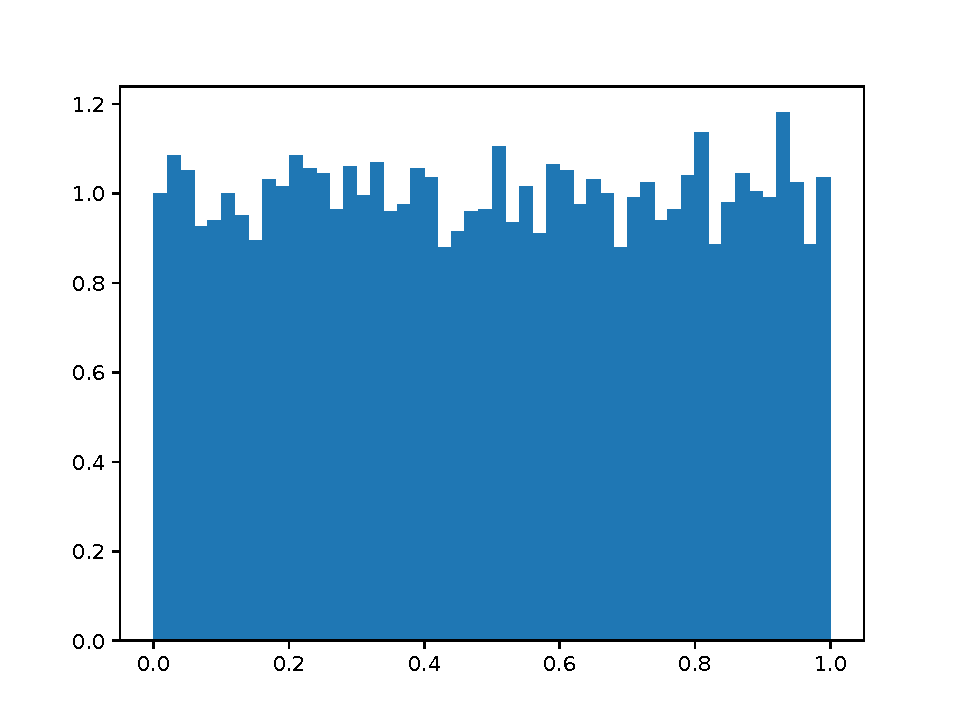
\includegraphics[width=0.4\linewidth]{sample_unif.pdf}
    \caption{Exemple de tirage uniforme sur $[0,\,1]$}
\end{figure}
\subsubsection{Addition homomorphe}\label{3.2.2} Supposons que l'on possède de deux chiffrés $\texttt{ct}_1$ et $\texttt{ct}_2$ de $\boldsymbol{m}_1$ et $\boldsymbol{m}_2$. Pour $\boldsymbol{u}_i \leftarrow \chi_{key}$, $\boldsymbol{e}_{i} \leftarrow \chi_{err}$;

    $$\texttt{ct}_1=\left(\left[\Delta[\boldsymbol{m}_1]_{t}+\boldsymbol{u}_1 \cdot \texttt{pk}_0+\boldsymbol{e}_{1}\right]_{q},\left[\boldsymbol{u}_1 \cdot \texttt{pk}_1+\boldsymbol{e}_{2}\right]_{q}\right) $$
    $$\texttt{ct}_2=\left(\left[\Delta[\boldsymbol{m}_2]_{t}+\boldsymbol{u}_2 \cdot \texttt{pk}_0+\boldsymbol{e}_{3}\right]_{q},\left[\boldsymbol{u}_2 \cdot \texttt{pk}_1+\boldsymbol{e}_{4}\right]_{q}\right)$$
L'addition de ces deux chiffrés fourni un nouveau chiffré, contenant un bruit dont les termes sont $\boldsymbol{e}_{1} + \boldsymbol{e}_{3},\, \boldsymbol{e}(\boldsymbol{u}_{1} + \boldsymbol{u}_{2})$ et $(\boldsymbol{e}_{2} + \boldsymbol{e}_{4})\boldsymbol{s}$, où $\boldsymbol{e} = \texttt{pk}_0 + \texttt{pk}_1 \boldsymbol{s}$.\\
Quand ces termes sont suffisamment grands et qu'un des coefficients du bruit est plus grand que $\Delta /2$, alors l'arrondi fournit un résultat faux et le déchiffrement est erroné. Le premier terme est une addition de polynômes dont les coefficients sont tirés selon une gaussienne discrète d'écart type $\sigma_{err}$. Si deux coefficients sont de signes opposés, le résultat va tendre vers zéro, sinon il sera plus grand. La figure \ref{addgauss} illustre la distribution de l'addition de $k$ polynômes de ce type, pour \colorbox{red}{}$k=2$, \colorbox{blue}{}$k=10$ et \colorbox{trolleygrey}{}$k=50$. Le cas général est donné par le Lemme 1 avec $\sigma(e_1 +\cdots+e_k) = \sqrt{k}\sigma_{err}$.
\begin{figure}[ht]
    \centering
    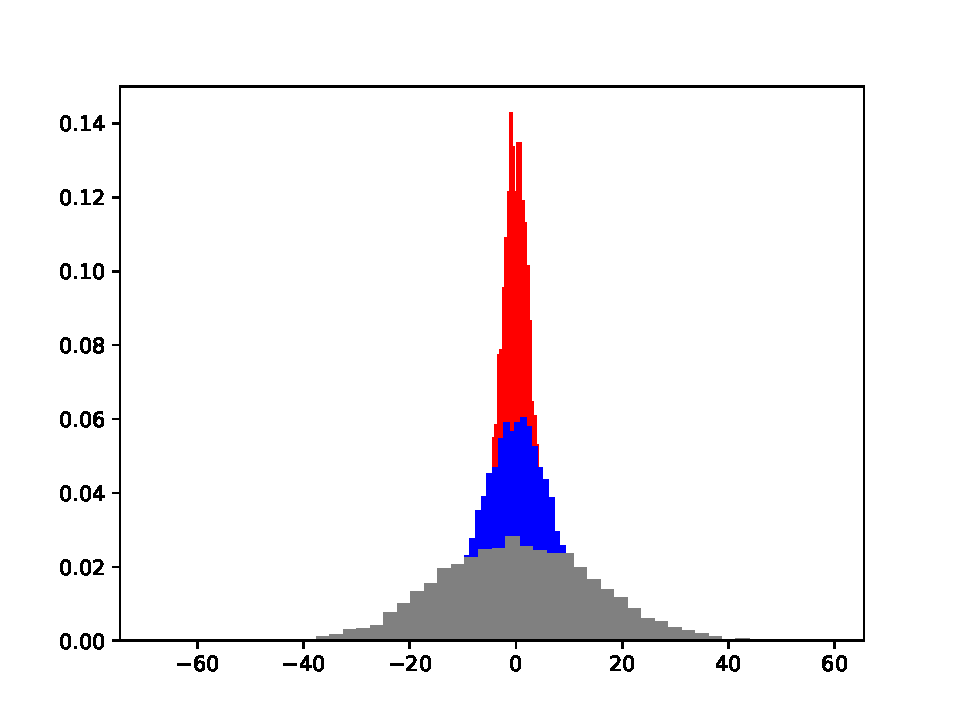
\includegraphics[width=0.45\linewidth]{add.pdf}
    \caption{\footnotesize{Addition de $k$ gaussiennes}}
    \label{addgauss}
\end{figure}

\begin{ex}
Pour $k=50$, certains coefficients du résultat peuvent aller jusqu'à la valeur $40$, il faut donc choisir un module $q$(et $t$), tel que $\Delta/2 > 40$, pour être certain que le déchiffrement soit correct.
\end{ex}
Le deuxième terme $\boldsymbol{e}(\boldsymbol{u}_{1} + \boldsymbol{u}_{2})$ est un produit d'une gaussienne par une addition de polynômes à coefficients dans $\{-1,0,1\}$. Comme la probabilité qu'un de ses coefficients soit non nul est de $\frac{2}{3}$, chaque coefficient du résultat sera l'addition d'au plus $\frac{2}{3}$ des coefficients de la gaussienne. Les coefficients du résultat sont plus importants que ceux du cas précédent (\textit{c.f.} [\ref{fig4-a}]), cette importance est due à l'addition des produits de coefficients, mais aussi à la réduction modulo $x^n + 1$, qui réduit la taille du polynôme résultant au prix d'une augmentation des coefficients (Ex: $20x^{n+5} - 30x^5 +1 \bmod x^n +1 = -50x^5 + 1$). $$\sigma(e\cdot(u_1 + \cdots u_k)) = \sqrt{\frac{2kn}{3}}\sigma_{err}$$

Enfin, le dernier terme $(\boldsymbol{e}_{2} + \boldsymbol{e}_{4})\boldsymbol{s}$ est similaire au deuxième. On multiplie la clé secrète, à coefficients dans $\{-1,0,1\}$ par une somme de gaussiennes. La figure [\ref{fig4-b}] illustre le comportement des coefficients du résultat, selon le nombre de gaussiennes additionnées. Soit $h$ le poids de Hamming de la clé secrète, égal au nombre de ses coefficients non nuls. On a 
$$\sigma(s\cdot(e_1 + \cdots e_k)) = \sqrt{hk}\sigma_{err}$$ 

\begin{figure}[ht]
  \centering
  \begin{subfigure}[b]{0.48\linewidth}
    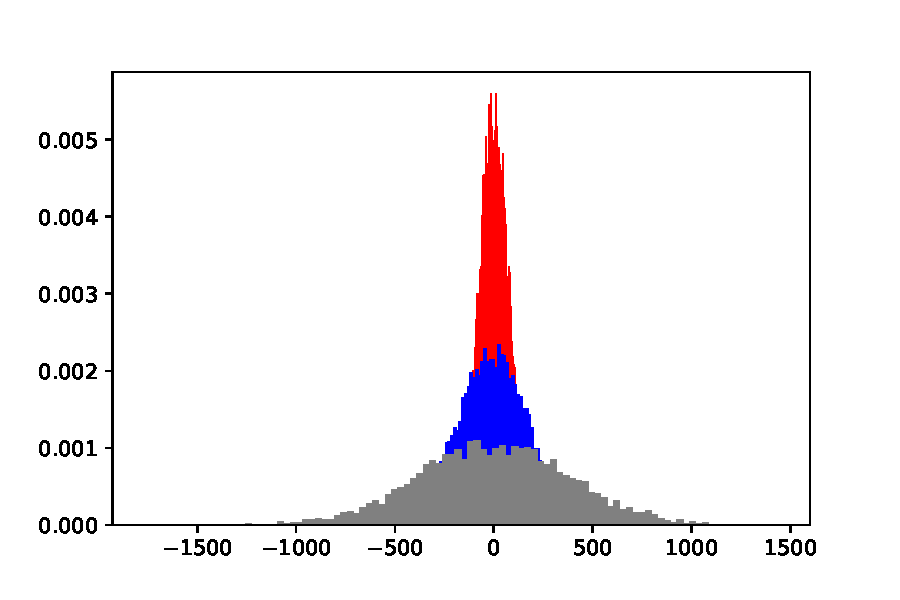
\includegraphics[width=\linewidth]{add2.pdf}
    \caption{\footnotesize{Multiplication d'une gaussienne par une\\ somme de $k$ polynômes à petits coefficients}}
    \label{fig4-a}
  \end{subfigure}
  \begin{subfigure}[b]{0.48\linewidth}
    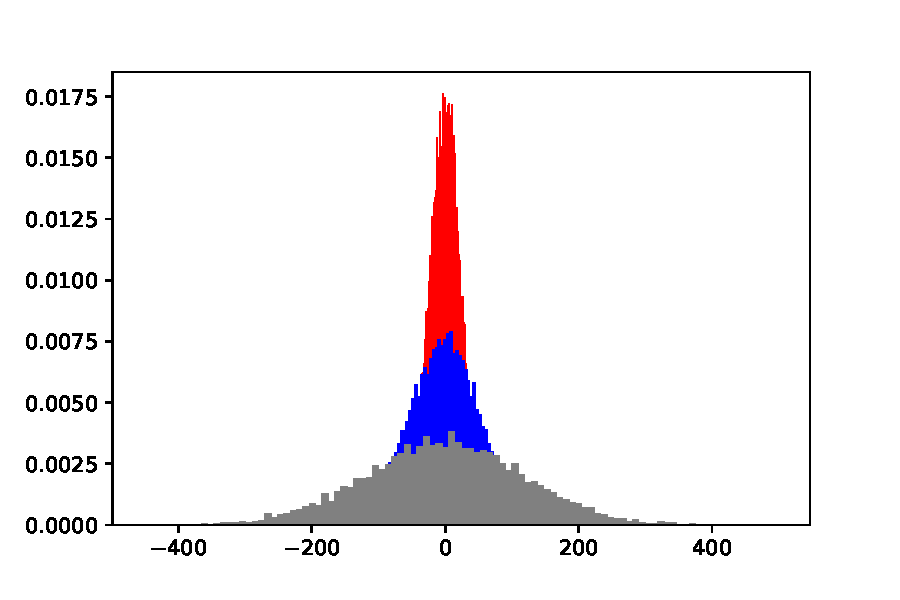
\includegraphics[width=\linewidth]{mul_key.pdf}
    \caption{\footnotesize{Multiplication d'un polynômes à petits\\ coefficients par une somme de $k$ gaussiennes}}
    \label{fig4-b}
  \end{subfigure}
\caption{}
\end{figure}

En combinant ces résultats, on remarque que le bruit peut être très important même quand on ne fait que des additions sur les chiffrés. Les paramètres $q$ et $t$ doivent êtres choisis selon le nombre d'additions à effectuer, de manière à ce que le rapport $q/t$ permette un déchiffrement correcte. L'écart type de la distribution obtenue après $k-1$ additions est $$\sigma_{\textrm{add}_k} = \left(\sqrt{k+\frac{2kn}{3}+ hk} \right)\sigma_{err}$$




\subsubsection{Multiplication homomorphe}
La multiplication de chiffrés entraîne une augmentation plus importante du bruit comparé à l'addition. On retrouve plusieurs termes de différents types dans le bruit du résultat.\\
Tout d'abord, commençons par donner une optimisation sur le facteur d'expansion. On considère les deux polynômes $\boldsymbol{a}(X) = \sum_{i=0}^{n-1} a_{i} X^{i}$ et $\boldsymbol{b}(X) = \sum_{i=0}^{n-1} b_{i} X^{i}$ de $\mathcal{R}$. Après multiplication, on obtient une borne $\|\boldsymbol{a}\cdot \boldsymbol{b}\|_{\infty} \leq n\|\boldsymbol{a}\|_{\infty}\|\boldsymbol{b}\|_{\infty}$ où $n$ représente, ici, le facteur d'expansion dans le pire des cas.

\begin{defi}
Soient $X_{1}, \ldots, X_{k}, k$ variables aléatoires indépendantes suivant $\mathcal{N}(0,\, 1)$, la variable $X =\sum_{i=1}^{k} X_{i}^{2}$ suit une loi $\chi ^2 _k$ à $k$ degré de liberté, sa densité de probabilité est $$f_{X}(x)=\frac{1}{2^{\frac{k}{2}} \Gamma\left(\frac{k}{2}\right)} x^{\frac{k}{2}-1} e^{-\frac{x}{2}},\, \forall x\geq0$$
avec $\Gamma : z \mapsto \int_{0}^{+\infty} t^{z-1} e^{-t} \mathrm{d}t$ la fonction gamma.
\end{defi}

la norme $\|\boldsymbol{a}\cdot \boldsymbol{b}\|_{\infty}$ atteint sa valeur en pire cas avec une probabilité négligeable, pour que cela arrive, il faut que tous les coefficients de $\boldsymbol{a}$(resp. $\boldsymbol{b}$) soient égaux à $\left\|\boldsymbol{a}\right\|_{\infty}$(resp. $\left\|\boldsymbol{b}\right\|_{\infty}$). Supposons $a_i, \, b_i$ tirés de $\mathcal{N}(0, \sigma ^2)$ et analysons la croissance de l'écart type $\sigma$. Pour tout $i$, le coefficient $\sum_{i=0}^{n-1} a_{i} b_{n-1-i}$  de $\boldsymbol{a}\cdot \boldsymbol{b}$ se comporte comme un échantillon de la distribution chi-square $\chi^2 _{2n}$ de degré de liberté $2n$, car pour tout $i$, on a $a_{i} b_{n-1-i}= \frac{1}{4}\left(a_{i}+b_{n-1-i}\right)^{2}-\frac{1}{4}\left(a_{i}-b_{n-1-i}\right)^{2}$.
\begin{figure}[ht]
  \centering
  \begin{subfigure}[b]{0.4\linewidth}
    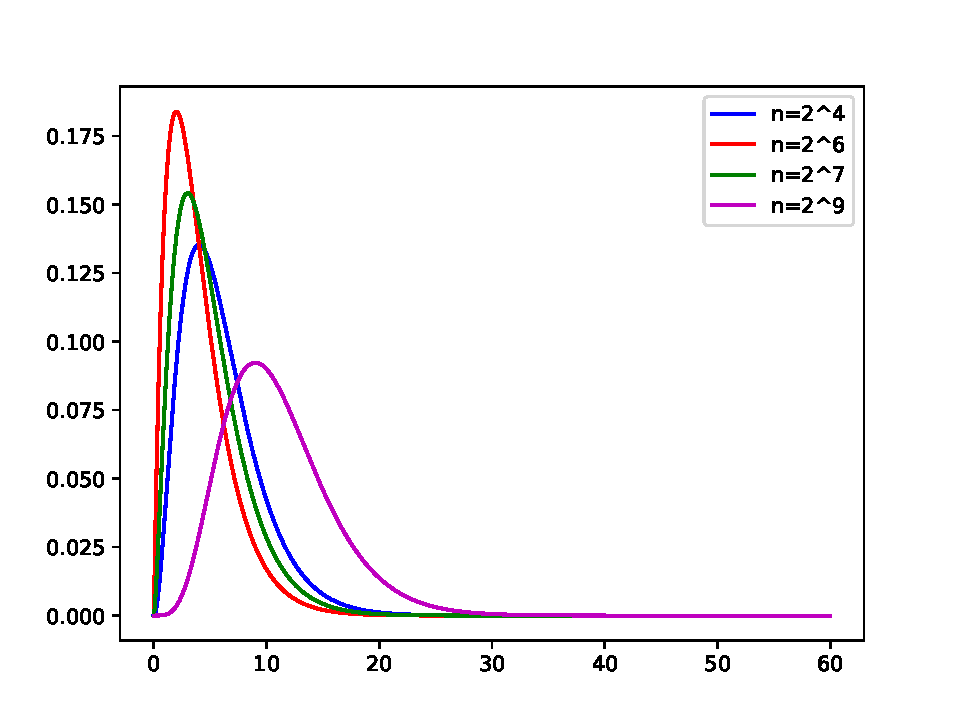
\includegraphics[width=\linewidth]{figure_1.pdf}
    \caption{PDF.}
  \end{subfigure}
  \begin{subfigure}[b]{0.4\linewidth}
    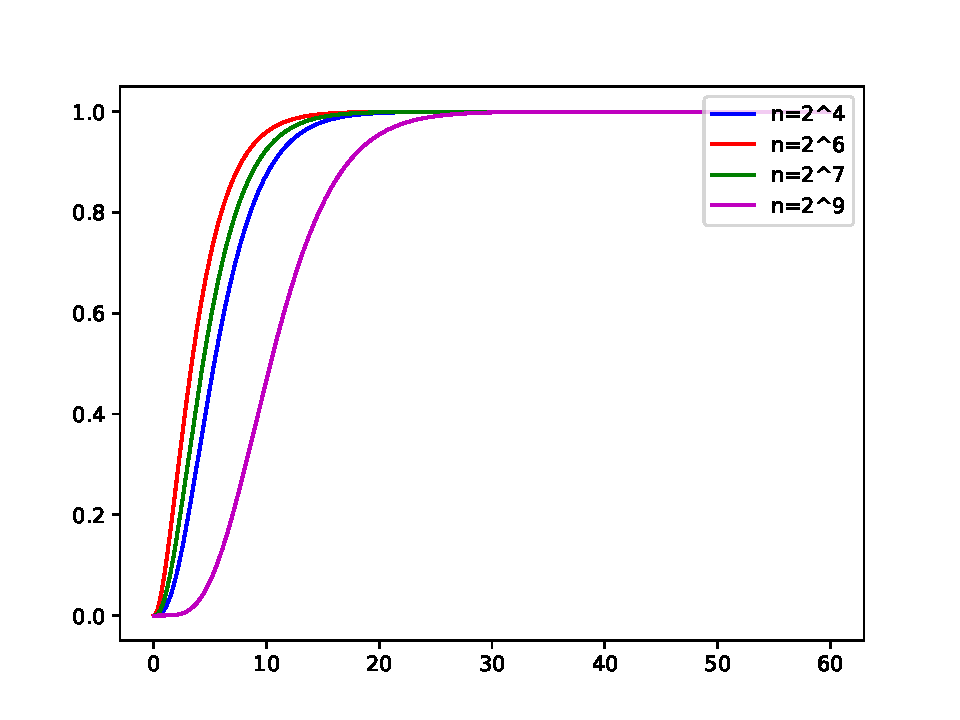
\includegraphics[width=\linewidth]{figure_2.pdf}
    \caption{CDF.}
  \end{subfigure}
  \caption{Loi de $\chi ^2 _n$}
  \label{fig:chi}
\end{figure}
\begin{theo}[Central Limite]
Soit $(X_i)_{1\leq i\leq n}$ une suite de variables aléatoires réelles indépendantes avec $\mathbb{E}(X_i)=\mu_i$ et $\operatorname{Var}(X_i) = \sigma_i ^2$ pour tout $i$. Alors, pour $n$ assez grand, la variable aléatoire $Z$ suit approximativement une loi normale $$Z=\frac{\sum_{i=1}^{n}\left(X_{i}-\mu_{i}\right)}{\sqrt{\sum_{i=1}^{n} \sigma_{i}^{2}}} \sim \mathcal{N}(0,\,1)$$
\end{theo}
Ainsi, pour $n$ assez grand ($2^9$ pour RLWE), $\chi^2 _{2n}$ tend vers une gaussienne de variance $4n$. Donc $$\sigma\left((\boldsymbol{a}\cdot \boldsymbol{b})_i = \sum_{i=0}^{n-1} a_{i} b_{n-1-i}\right) \approx \sqrt{n} \sigma^{2}$$
\begin{rem}\label{rem7}
Si $\boldsymbol{a}$ est un polynôme constant et les coefficients $b_i$ tirés de $\mathcal{N}(0, \sigma_b ^2)$, par le Lemme 1 on a $\sigma_{ab} =\sqrt{\sum_{i=0}^{n-1} (a_{i} \sigma_b)^2} = \sigma_b \|\boldsymbol{a}\|_2$.
\end{rem}
Le résultat de cette remarque peut servir lorsque le bruit est multiplié par un clair, on obtient $\sigma([\boldsymbol{m}]_t \cdot\boldsymbol{v}) = \|\boldsymbol{m}\|_2\sigma_{\boldsymbol{v}} \leq \sqrt{n} \sigma_{\boldsymbol{v}}$ pour un message à coefficients binaires.\\

Ensuite, revenons à l'écriture $\texttt{ct}_i (s) = \Delta\boldsymbol{m}_i + \boldsymbol{v}_i + q\boldsymbol{r}_i$, le bruit $\boldsymbol{r}_i$ résulte principalement d'un produit entre un polynôme à coefficients uniformes sur $[-1/2,\,1/2)$ (division par $q$ de l'uniforme sur $[-q/2,\,q/2)$) et la clé secrète $\boldsymbol{s}$, dont les coefficients sont tirés aléatoirement de l'ensemble $\{-1,\,0,\,1\}$. Ce bruit est majoré, dans le pire cas, par  $\|\boldsymbol{r}_i\|_\infty \leq \frac{1}{2t}+ \frac{\delta_\mathcal{R} B_{key}}{2} + 1$. Soit $h$ le poids de Hamming de $\boldsymbol{s}$ et $(\boldsymbol{a}\cdot\boldsymbol{s})_i = \sum_{i=0}^{n-1} u_{i} s_{n-1-i}$ le $i$-ème coefficient du produit. Comme tous les $a_i$ ont une variance $\operatorname{Var}(a_i) =\frac{1}{12}$, alors $\operatorname{Var}((\boldsymbol{a}\cdot\boldsymbol{s})_i) = h \times \operatorname{Var}(a_i) = \frac{h}{12}$.\\
\begin{figure}[ht]
  \centering
  \begin{subfigure}[t]{2.5in}
  \centering
    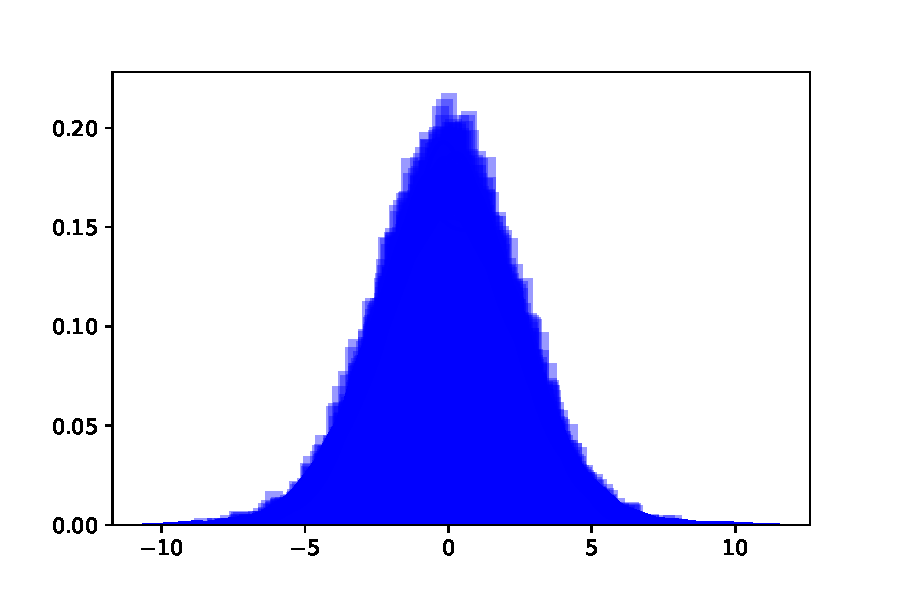
\includegraphics[width=\linewidth]{prod.pdf}
    \caption{\footnotesize{La distribution des coefficients de $\boldsymbol{a}\cdot\boldsymbol{s}$,\\où $\boldsymbol{s}$ est tirée en fonction de son poids de\\ hamming $h$}}
  \end{subfigure}
  \begin{subfigure}[t]{2.5in}
  \centering
    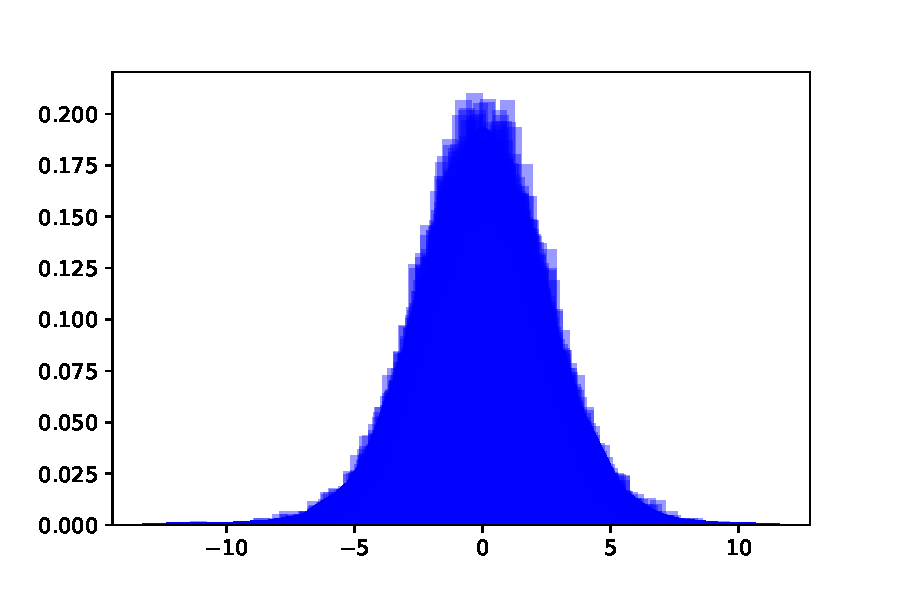
\includegraphics[width=\linewidth]{ham.pdf}
    \caption{\footnotesize{Gaussienne d'écart type $\sqrt{\frac{h}{12}}$, pour $h=63$.}}
  \end{subfigure}
 \caption{\footnotesize Estimation du bruit $\boldsymbol{r}_i =\dfrac{1}{q}(\texttt{ct}_i (s) - \Delta\boldsymbol{m}_i - \boldsymbol{v}_i$)}
\label{fig:6}
\end{figure}

On reprend l'écriture des deux chiffrés utilisés pour l'addition et on se met dans le cas optimal, on a $\boldsymbol{v}_{mult_1} = \boldsymbol{m}_{1} \cdot \boldsymbol{v}_{2}+\boldsymbol{m}_{2}\cdot\boldsymbol{v}_{1}+t\left(\boldsymbol{v}_{1} \cdot \boldsymbol{r}_{2}+\boldsymbol{v}_{2} \cdot \boldsymbol{r}_{1}\right) + \epsilon$, pour $\epsilon$ très petit. Analysons le comportement du terme 
$(\boldsymbol{m} + t\boldsymbol{r})(\boldsymbol{e}_{1} + \boldsymbol{e}_{3} + \boldsymbol{e}\cdot(\boldsymbol{u}_{1} + \boldsymbol{u}_{2}) + (\boldsymbol{e}_{2} + \boldsymbol{e}_{4})\cdot\boldsymbol{s})$, où $\boldsymbol{r}$ est d'écart type $\sqrt{\frac{h}{12}}$. Par le Lemme \ref{lem1}, $t\boldsymbol{r}$ est une gaussienne $\boldsymbol{r}^\prime$ d'écart type $\sigma_{r^\prime} = \sqrt{\frac{ht}{12}}$, qui sera multipliée par l'expression du bruit après une addition. D'après une expérience similaire au (\ref{3.2.2}) sur 500 échantillons, pour $t=2$, $n=1024$, $h=63$, $\sigma_{err} = 3.2$ \cite{fan2012somewhat}, \cite{Cingulata} et les $\boldsymbol{u}_i$ avec $\frac{2n}{3}$ coefficients non nuls.

\begin{Bilan}
La multiplication de deux chiffrés de degré 1 en $\boldsymbol{s}$, dont le bruit est tiré selon une gaussienne d'écart type $\sqrt{\frac{2n}{3}+h+1} \cdot \sigma_{err}$, est un chiffré de degré 2, contenant un bruit suivant $\mathcal{N}(0,\,\sigma_{mult_1} ^2)$ avec
$$\sigma_{mult_1} = \sqrt{n}\sqrt{\frac{nht}{18} + \frac{ht}{12}(1+h)} \cdot \sigma_{err}$$
Le carré de cette valeur est inférieur à la borne donnée dans (\ref{eq:12}). 
\end{Bilan}

\begin{figure}[ht]
  \centering
  \begin{subfigure}[t]{2.5in}
    \hfill
    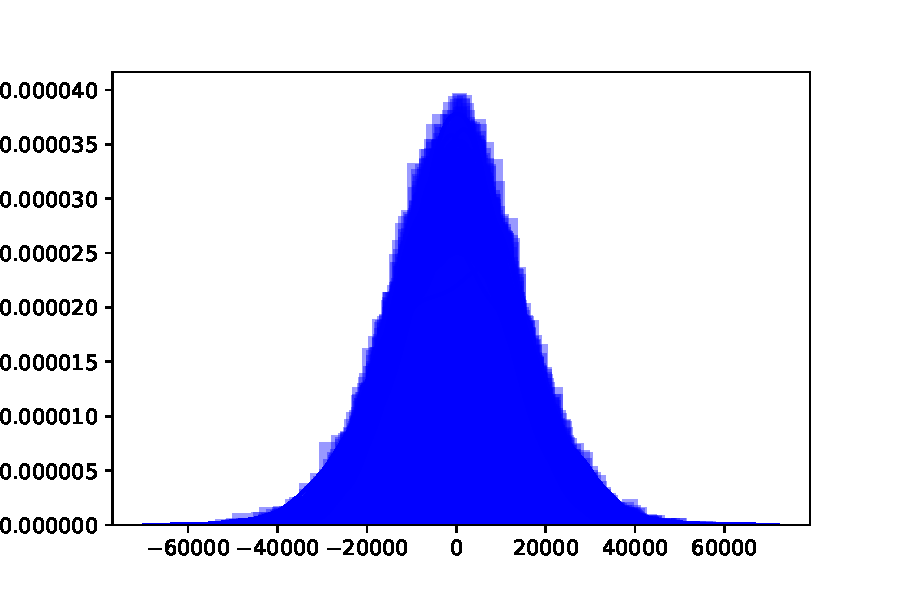
\includegraphics[width=\linewidth]{one_mult.pdf}
    \subcaption{\footnotesize La distribution des coefficients après\\une seule multiplication}
    \label{fig7-a}
  \end{subfigure}
  \begin{subfigure}[t]{2.5in}
    \hfill
    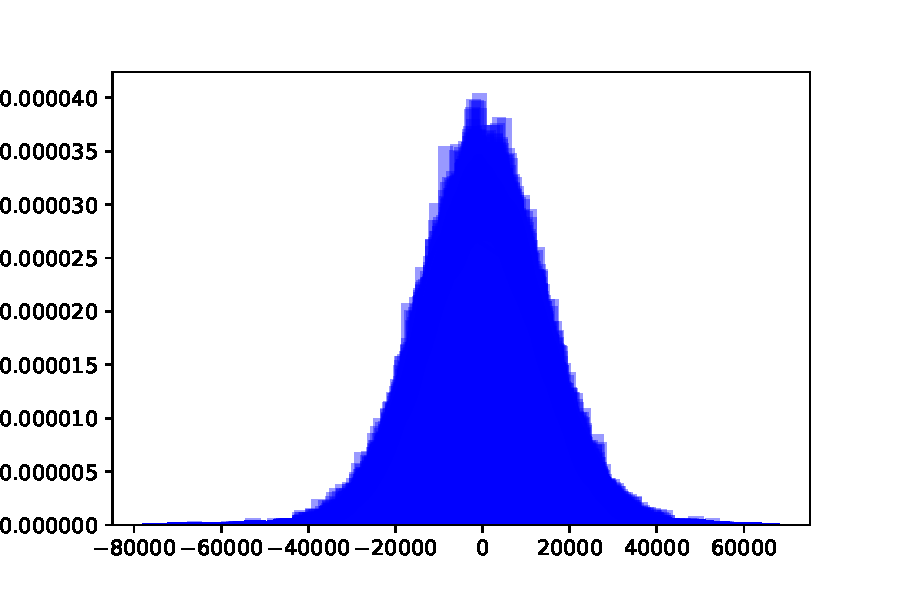
\includegraphics[width=\linewidth]{optim.pdf}
    \subcaption{\footnotesize Distribution d'écart type $\sqrt{n}\sigma_{\textrm{add}_2} \sigma_{r^\prime}$}
    \label{fig7-b}
  \end{subfigure}
\caption{Comparaison des estimations théoriques et les résultats des simulations}
\end{figure}

La situation change quand on fait deux multiplications. En effet, si on multiplie le résultat de la multiplication par un troisième chiffré, on se retrouve avec un bruit de la forme $\boldsymbol{v}_{mult_2} = (\boldsymbol{m}_{1}\cdot \boldsymbol{m}_{2})\cdot\boldsymbol{v}_{3}+\boldsymbol{m}_{3} \cdot\boldsymbol{v}_{mult_1}+t\boldsymbol{r}\left(\boldsymbol{v}_{mult_1}  +\boldsymbol{v}_{3}\right)$. Or les coefficients du produit de deux messages binaires peuvent atteindre $\sqrt{n}$. Il est donc indispensable de considérer le nombre de coefficients non nuls pour chaque message $\boldsymbol{m}_i$.\\

Une analyse similaire à \cite{cryptoeprint:2016:254} en utilisant la Remarque \ref{rem7} donne le résultat suivant
\begin{prop}
Soient $\texttt{ct}_i$ pour $1\leq i \leq k+1$ des chiffrés de $\boldsymbol{m}_i$, contenant des bruits $\boldsymbol{v}_i$ de $\mathcal{N}(0,\,\sigma_i ^2)$. $\texttt{ct}_f$ est le résultat d'une chaîne de $k$ multiplications 
$$\texttt{ct}_{f}=\texttt{FV.Mult}\left(\texttt{ct}_{1},\, \texttt{FV.Mult}\left(\texttt{ct}_{2},\,\texttt{FV.Mult}\left(\dots,\, \texttt{FV.Mult}\left(\texttt{ct}_{k},\, \texttt{ct}_{k+1}\right)\right) \right) \right)$$
de bruit $\boldsymbol{v}_f$ suivant $\mathcal{N}(0,\,\sigma_f ^2)$ avec 

$$\begin{aligned}
\sigma_f ^2 &= \sigma_1 ^2 \prod_{i=2}^{k+1}(N_i ^2 + \alpha^2) + \sigma_2 ^2 \prod_{i=1,\,i\neq2}^{k+1}(N_i ^2 + \alpha^2) \\&+{\sum_{j=3}^{k} \sigma_j ^2(\prod_{i=j+1}^{k+1} (N_i ^2 + \alpha^2))((\prod_{i=1}^{j-1} N_i )^2 + \alpha^2 )} \\&+ { ((\prod_{i=1}^{k} N_i )^2 + \alpha^2 )\sigma_{k+1} ^2}
\end{aligned}$$
où $N_i = \left\|\boldsymbol{m}_i \right\|_2$ et $\alpha = \sqrt{n}\sigma_{\boldsymbol{r}^\prime} = \sqrt{nht/12}$. Pour un message $\boldsymbol{m}_i$ à coefficients binaires, $N_i ^2$ représente le nombre de coefficients non nuls.

\end{prop}
Ce résultat est obtenu par récurrence sur le nombre de multiplications $k$. La procédure de relinéarisation n'a pas été utilisée ici mais il est facile de l'inclure, soit en l'utilisant après chaque multiplication de chiffrés de degré 1 en $\boldsymbol{s}$, ou bien après avoir atteint le nombre d'opérations souhaité. Cette procédure n'est pas nécessaire pour assurer l'exactitude de la multiplication homomorphe.

\subsubsection{La probabilité d'échec}
Soit $\mathcal{B}$ la nouvelle borne avec les optimisations, en acceptant la possibilité que le déchiffrement puisse être erroné avec une probabilité négligeable, on peut prendre un module $q$ plus petit que celui donné par la borne en pire cas. Si on suppose $\Delta/2 > x\mathcal{B}$ avec une marge d'erreur $x>1$, la probabilité que la norme d'un seul coefficient de $\boldsymbol{a}\cdot \boldsymbol{b}$ dépasse $x\sigma$ est $\mathbb{P}\left(\left|\sum_{i=0}^{n-1} a_{i} b_{n-1-i}\right|>x \sigma\right) = 1-\operatorname{erf}(x / \sqrt{2})$, avec $\operatorname{erf}(x)=\frac{2}{\sqrt{\pi}} \int_{0}^{x} e^{-t^{2}} \mathrm{d} t$ la fonction d'erreur. Si on suppose que tous les coefficients sont indépendants, alors $$\mathbb{P}\left(\left\|\boldsymbol{a}\cdot\boldsymbol{b}\right\|_{\infty}>x \sigma\right) = \left(1-\operatorname{erf}(x /\sqrt{2})\right)^n$$

\section{Le choix des paramètres}
Le choix des paramètres pour les schémas homomorphes reposant sur le problème RLWE est toujours un sujet de recherche, la tâche étant d'améliorer leur efficacité, tout en garantissant une sécurité prouvée. Il n'y a pas encore de recommandations officielles pour choisir des paramètres avec des niveaux de sécurité standards. Dans cette section, on présentera les algorithmes utilisés pour générer les paramètres d'un schéma homomorphe reposant sur le RLWE, ainsi qu'une comparaison avec notre approche.

\subsection{Paramètres du schéma FV}
Un schéma SHE, en particulier FV, peut évaluer un circuit arithmétique d'une profondeur multiplicative prédéterminée $L$, cette restriction ayant pour objectif de garantir le déchiffrement soit correct après un certain nombre d'opérations. Les paramètres sont ainsi choisis de façon à ce que le bruit reste inférieur à la borne de déchiffrement pour des circuits de profondeur allant jusqu'à la valeur choisie $L$. Cependant, la complexité de chaque opération homomorphe augmente également avec $L$. De plus, la profondeur multiplicative ne prend pas en compte le bruit des additions, ce qui peut conduire à la perte des données claires.\\
Les travaux actuels, notamment Migliore et al. \cite{migliore:hal-01394362}, décrivent un algorithme de génération des paramètres selon le niveau de sécurité souhaité $\lambda$ et la profondeur multiplicative $L$. Pour des valeurs arbitraires pour le degré du polynôme cyclotomique $n$, la fonction \texttt{ChooseParam(FV,$L$,$\lambda$)} calcule $\sigma > 2\sqrt{n}$, une borne maximale $q_{max}$ pour le module $q$ selon ($\lambda$, $n$) et enfin une borne minimale $q_{min}$ compatible avec $L$ (garantit un déchiffrement correcte). Si $q_{max} < q_{min}$, on prend $n$ plus grand et on recommence. Il existe une autre approche où l'on choisit $\sigma = \frac{\alpha q}{\sqrt{2\pi}} \simeq 3.2$ (le paramètre de sécurité $\alpha$ est tel que $\alpha q \simeq 8$) \cite{HomomorphicEncryptionSecurityStandard}.
Un autre outil facilitant le choix des paramètres a été développé au CEA-List (CinguParam \cite{CinguParam}), dédié aux implémentations \cite{sealcrypto,Cingulata, FV-NFLlib}. Il utilise le LWE-Estimator\footnote{\url{https://bitbucket.org/malb/lwe-estimator/src/master/}} \cite{cryptoeprint:2015:046} qui permet d’évaluer la sécurité des instances LWE, en considérant les meilleurs attaques connues (attaques LWE \cite{cryptoeprint:2015:1092,HomomorphicEncryptionSecurityStandard}), contre les systèmes de chiffrement reposant sur le RLWE. Cet outil permet ainsi de comparer l’impact des choix de paramètres pour les systèmes homomorphes et de mesurer l’incertitude sur le niveau de sécurité concret.\\
Cependant, ces outils utilisent des bornes pessimistes \cite{fan2012somewhat} pour pouvoir générer des paramètres assurant un déchiffrement correcte, ce qui nuit aux performances. Dans notre approche, on estime la variance totale de n'importe quel circuit grâce aux formules d'addition et de multiplication, ce qui nous permettra, d'un coté, de prendre en compte le bruit des additions, mais aussi de traquer le bruit le long du circuit.

\subsubsection{Paramètres assurant un déchiffrement correct}

\subsubsection{Paramètres assurant la sécurité}
\subsection{Résultats expérimentaux}



\section{Bootstrapping}
L. Ducas et D. Micciancio \cite{cryptoeprint:2014:816} ont construit un schéma, appelé FHWE et avec lequel le bootstrapping peut être effectué en moins d'une seconde. Ce schéma a été amélioré par I. Chillotti et al pour devenir le TFHE \cite{TFHE}, reposant sur une variante du RLWE sur le tore réel. Le bootstrapping peut ainsi être effectué en 0.1 secondes.

\newpage
\footnotesize
\nocite{*}    
\bibliographystyle{alpha}
\bibliography{fhe}
\end{document}